We use the HPS detector simulation system based on SLAC's org.lcsim infrastructure for full GEANT4
simulation of the passage and interaction of charged and neutral particles through the SVT 
and the ECal to the muon detector. In the SVT, the simulation creates realistic energy deposits in the silicon 
microstrip detectors, accounts for dead material, simulates APV25 signal sampling every 25 ns, 
creates clusters, and performs track finding and reconstruction.
In the ECal, the geometry for the flange and vacuum chamber is based on a tessellated 
representation imported directly from the CAD drawings. It creates energy deposits in individual 
trapezoidal-shape $PbWO_4$ crystals, simulates FADC signal time evolution and sampling every 4 ns, and 
generates triggers based on the  FPGA trigger algorithm implementation.
To maintain the chicane beamline configuration, the field strength of the
chicane magnets must scale with the beam energy. The performance studies were 
made using the field strength of the 
analyzing magnet of 0.25 Tesla at 1.1 GeV, 0.5 Tesla at 2.2 GeV, and 
1.5 Tesla at 6.6 GeV.
Figure  \ref{fig:lcsim} shows a lcsim rendering of the HPS detector.

\begin{figure}[h]
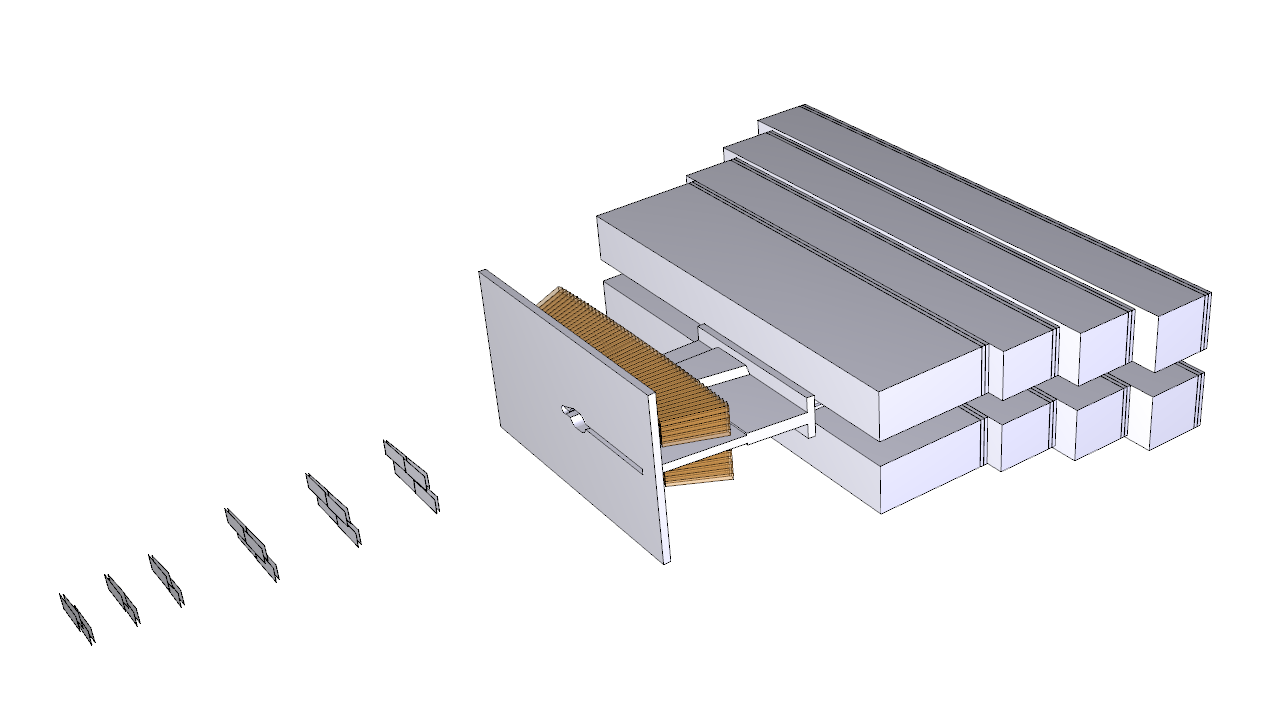
\includegraphics[width=\textwidth]{performance/lcsimDetector}
\caption{\small{ Rendering of the HPS detector simulation}}
\label{fig:lcsim}
\end{figure}

\subsection{Simulation of backgrounds and detector occupancies}

\subsubsection{Simulation of backgrounds}
\label{sec:backgrounds}

The multiple Coulomb scattering and bremsstrahlung processes in the target will generate high 
intensity fluxes of electrons and photons in the very forward direction, while the large
M{\o}ller interaction cross section with atomic electrons will generate high intensity low energy
electrons. We use the high energy interaction simulation tools GEANT4 and EGS5 to simulate 
these backgrounds. In the original HPS proposal to JLab PAC37 \cite{HPS_PROP}, we described a significant 
disagreement between these tools. GEANT4 predicted a broader angular
distribution of multiple scattered electrons than EGS5, resulting in twice the occupancy in the
tracker near the dead zone and much higher ECal trigger rates. 
The HPS Test run was motivated in part by the need to resolve this discrepancy, and the outcome of the test run is described 
in the previous section. The algorithms used 
in the codes to simulate the multiple scattering have been studied, and the findings are summarized in
Appendix \ref{app:sim}. The test run result and the algorithm studies have confirmed that EGS5 can describe the multiple scattering 
tails more accurately than GEANT4. All the electromagnetic interactions in the target are simulated with EGS5.   

When bound electrons in the target are ionized by incoming electrons or secondary photons, outer 
shell electrons will fill the vacancy and characteristic X-rays are emitted. 
These X-rays can contribute background hits in
the SVT when a conversion takes place in the silicon sensors via the photoelectric effect 
or Compton scattering. Since X-ray production from electrons interactions is not fully simulated in EGS5, we estimate the X-ray intensity at SVT layer 1 using the impact ionization cross section, $\sigma_I$, \cite{hoffmann}, the fluorescence yield, $\omega$, \cite{hubbell},
the photoabsorption length in Tungsten, $\lambda_W$, to account for the self-absorption, and the solid 
angle of the SVT layer 1.
Table \ref{tab:xray} summarizes these parameters and the expected X-ray
fluxes at SVT Layer 1 for 0.25\% $X_0$ Tungsten and 100 nA beam current in 8 nsec time window. 
X-ray backgrounds are not a concern.

\begin{table}[h]
\begin{center}
\begin{tabular}{|c|c|c|c|c|c|} \hline
  & Energy (keV) & $\sigma_I$ (barns) & \hspace{0.5 cm} $\omega$ \hspace{0.5 cm} & $\lambda_W$ ($\mu$m) & $N_\gamma$ at Layer 1 in 8 ns   \\ \hline
K-shell & 60 & 40 & 0.95 & 100 & 0.5 \\ \hline
L-shell  & 10 & 1000 & 0.30 & 5 & 2 \\ \hline
M-shell  & 2 & 20000 & 0.02 & 0.2 & 0.1 \\ \hline
\end{tabular}
\end{center}
\caption{\small{X-ray intensities}}
\label{tab:xray}
\end{table}

Hadrons are also produced in the target. Hadron production is at least three orders
of magnitude smaller than the electromagnetic interaction. The polar angle for hadron production
is predominantly larger than 100 mrad, whereas the HPS detector acceptance is limited to less than
100 mrad. Furthermore, the hadron energy spectrum is soft as they are produced from the 1/k bremsstrahlung
spectrum and more than 90\% of the hadrons are swept away by the analysing magnet before reaching the ECal.
 The hadron production is simulated using GEANT4 and FLUKA. In a target thinner than
about 5\% $X_0$, the ``virtual'' photon interaction is dominant \cite{mohring}. The inclusive hadron
production ${\sigma (eA\rightarrow X)}$ is simulated from the photonuclear process ${\sigma (\gamma A
\rightarrow X)}$ using the equivalent photon approximation,

$$ \sigma (eA \rightarrow X) = \int \sigma_k(\gamma A \rightarrow X) dn(k), $$

\noindent
where $dn(k)$ is the number of equivalent photons with energy $k$ \cite{budnev} and there are 
approximately $8 \times 10^{10} $ photons/sec in 6.6 GeV 100 nA beam. 
Table \ref{tab:pion} summarizes the pion single rates from 1\% $X_0$ Tungsten target
and 6.6 GeV 100 nA beam. While pion production is larger in GEANT4, the energy spectrum is softer and
consequently the single rate of pions reaching the ECal is lower in GEANT4. While pions look like a minimum 
ionizing particle in the ECal most of the time, they can deposit significant energy when ${\pi^0}$ are
produced in the ECal crystals, and together with the beam background, they contribute accidental coincident triggers. 

\begin{table}[h]
\begin{center}
\begin{tabular}{|c|c|c|} \hline
  & Total production rate (kHz) & Single rate reaching the ECal (kHz) \\ \hline
GEANT4 & 410 & 8 \\ \hline
FLUKA  & 240 & 15 \\ \hline
\end{tabular}
\end{center}
\caption{\small{Pion single rates from 1\% $X_0$ Tungsten target at 6.6 GeV 100 nA}}
\label{tab:pion}
\end{table}

\pagebreak
\noindent
Other beam induced background we considered are:

\begin{itemize}
\item
Beam halo

Beam halo was measured using a large dynamic range halo monitor during the 6 GeV era. The beam halo 
that extends to 2 mm was found at the level of $10^{-7}$. At this level, the halo contribution in 
the SVT occupancy is negligible. It is expected that behavior of the 12 GeV machine will be
understood at the same level.

\item
Synchrotron radiation

Synchrotron radiation is produced from the last dipole magnet in the beam line in the vertical 
plane, and from the chicane magnets in the horizontal plane. Since the characteristic energy is 
proportional to $E_{beam}^2$, synchrotron radiation is of concern 
only at 6.6 GeV. The characteristic energy ($k_c$),
the average energy ($k_{ave}$), and the power of the synchrotron radiation is summarized in 
Table \ref{tab:sync}.
None of the radiation from the last dipole will enter the HPS detector as the radiation will be intersected 
by the beamline collimator. The radiation from the chicane magnets is in the dead zone, and
none of the detector components are designed to intersect the beam plane.   

\begin{table}[h]
\begin{center}
\begin{tabular}{|l|c|c|c|c|} \hline
  Source & $k_c$ (keV) & $k_{ave}$ (keV) & $N_\gamma$ per e- & Power (mW) at 100 nA \\ \hline
  vertical bend & 19 & 5.9 & 4.0 & 2.4 \\ \hline
  Frascati Magnet & 52 & 16 & 4.6 & 7.4 \\ \hline
  PS magnet   & 44 & 14 & 9.3 & 13 \\ \hline
\end{tabular}
\end{center}
\caption{\small{Synchrotron radiations at 6.6 GeV}}
\label{tab:sync}
\end{table}


\item
EM induced backgrounds

Electromagnetic fields induced by the high intensity beam could interfere with the SVT and its electronics
as the detector is located as close as 0.5 mm from the beam. We have evaluated the direct beam field and its wake 
field, the diffraction radiations from the beamline apertures, and the transition radiations from
the target. The intensities of these EM induced backgrounds are small and no interference with the SVT is expected. The beam charge per 2ns CEBAF bunch is only ~few thousand electrons, many orders of magnitude lower than that in other experiments which have chosen to shield against it.
 
\end{itemize}

\subsubsection{Simulated Tracker Occupancies}

Figure \ref{fig:scatt} shows the distribution of charged particle hits in Si tracker layer 1 
which is located 
10 cm from the target. The beam energy is 6.6 GeV, and the target thickness is 
0.25\% $X_0$. Multiple Coulomb scattered beam electrons are confined to within 0.5 cm of the beam axis
(x=y=0), while the low energy M{\o}ller electrons are distributed in a parabolic shape. There are
very few positrons. From these distributions, the detector occupancy in the horizontal Si strip
sensor in the 8 ns time window is calculated for a 400 nA beam current and five different target
thicknesses, 1.0\% $X_0$, 0.5\% $X_0$, 0.25\% $X_0$, 0.1\% $X_0$, and 0.05\% $X_0$, as shown
in Figure \ref{fig:occup}. 
%As described in Section xx, the dead zone is defined by using a criterion that the maximum occupancy in Layer 1 is 1\%. 
For a 0.25\% $X_0$ target and 430 nA beam, the occupancy is 
1\% at a distance of 1.5mm from the beam in Layer 1, which corresponds to a dead zone of $\pm$ 15
mrad. As long as the product of target thickness (T) and beam current (I) is constant, the same 
$A'$ production rate is maintained. Since multiple scattering and hence the effective beam size 
is reduced in a thinner target, it is advantageous to use a thinner target and a higher current.
Using the constraint that the occupancy is 1\% at 15 mrad, we find the beam current $I$ which 
gives this occupancy for each of several potential target thicknesses $T$. The quantity 
$(I\cdot T)^{1/2}$, which is approximately proportional to the sensitivity $S/\sqrt{B}$, is
given in Table \ref{tab:occup}, showing how the sensitivity improves as the target thickness 
decreases.

\begin{figure}[h]
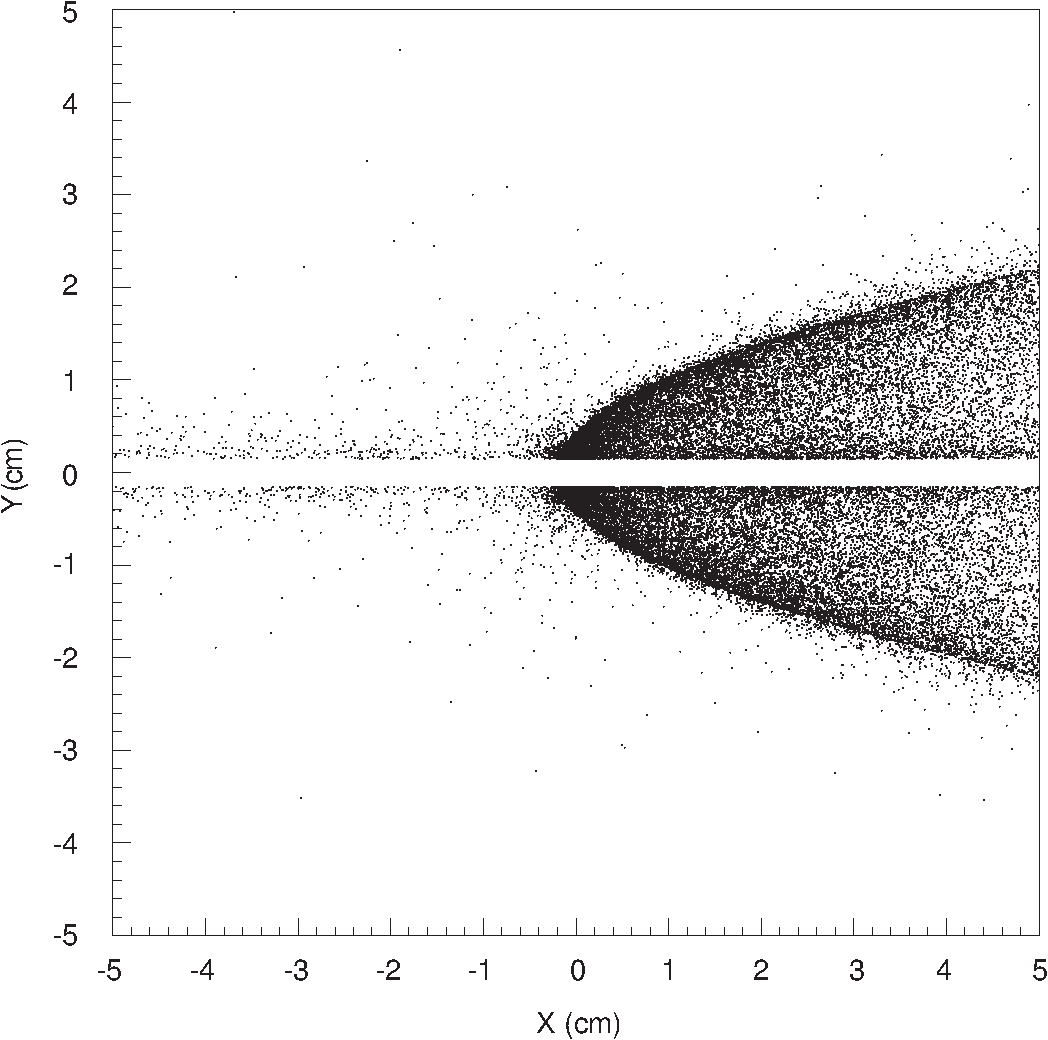
\includegraphics[width= 0.7\textwidth]{performance/scatterplot.pdf}
\caption{\small{Charged particle distribution in SVT layer 1.}}
\label{fig:scatt}
\end{figure}

\begin{figure}[t]
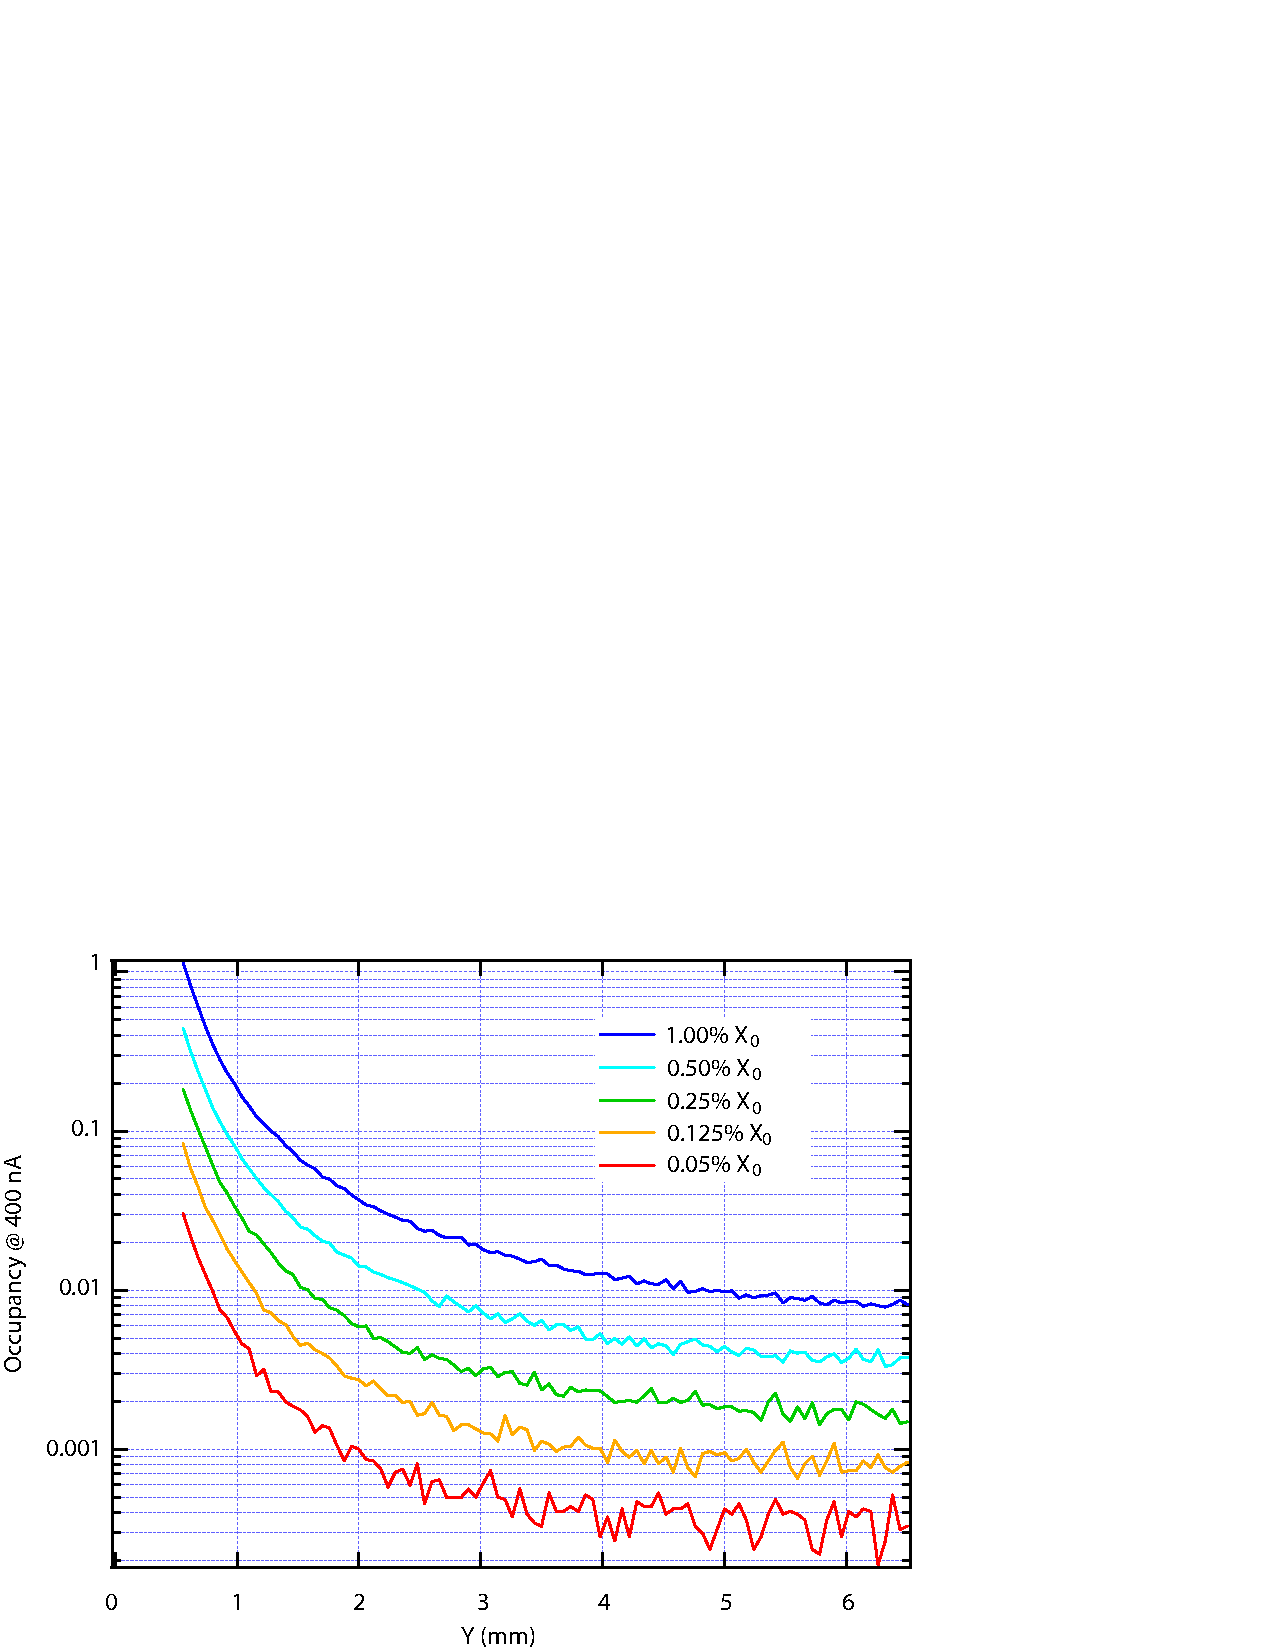
\includegraphics[width=0.8\textwidth]{performance/occupancy.pdf}
\caption{\small{Silicon sensor layer 1 occupancy at 400 nA vs. distance from the
beam in mm.}}
\label{fig:occup}
\end{figure}

\begin{table}[h]
\begin{center}
\begin{tabular}{|c|c|c|} \hline
  Target thickness (\% $X_0$) & Beam Current (nA) & $\propto S/\sqrt{B}$ \\ \hline
  1.0 & 60 & 7.7 \\ \hline
  0.5 & 170 & 9.1 \\ \hline
  0.25 & 430 & 10.4 \\ \hline
  0.10 & 1330 & 11.6 \\ \hline
  0.05 & 2860 & 11.9 \\ \hline
\end{tabular}
\end{center}
\caption{\small{Beam current yielding 1\% occupancy in SVT layer 1 for various target 
thicknesses at 6.6 GeV, and the relative experimental sensitivities which result.}}
\label{tab:occup}
\end{table}

The run conditions for other possible beam energies are studied using the same criterion that the maximum occupancy 
in SVT Layer 1 does not exceed 1\%. Table \ref{tab:runc} summarizes the target thickness and proposed beam current. 

\begin{table}[h]
\begin{center}
\begin{tabular}{|c|c|c|} \hline
  Beam Energy & Target thickness (\% $X_0$) & Beam Current (nA) \\ \hline
  1.1 & 0.125 & 50 \\ \hline
  2.2 & 0.125 & 200 \\ \hline
  4.4 & 0.25  & 300 \\ \hline
  6.6 & 0.25 & 450 \\ \hline
\end{tabular}
\end{center}
\caption{\small{Run Conditions}}
\label{tab:runc}
\end{table}

\clearpage

\subsubsection{Simulated ECal occupancies}

There are two factors limiting the allowable ECal occupancy. First, the ECal 
readout algorithm uses a window of fixed size to integrate hit energy. This 
window was set to 140 ns ($35 \times 4$ ns) for the test run, and so the 
number of hits above readout threshold in a 140-ns time window should be well 
below 1. Figure \ref{fig:ecal_rate} shows that the maximum rate in any crystal 
is 500 kHz, which translates to 0.07 hits in 140 ns.

Second, because the FADC only reads out on a rising threshold crossing, each 
hit above threshold causes dead time for that crystal until the preamp output 
falls back below threshold. Figure \ref{fig:ecal_deadtime} shows the fraction 
of time each crystal spends above threshold. The maximum dead time is 0.03, 
meaning that even the hottest crystal is sensitive to new hits 97\% of the time.

\begin{figure}[ht]
	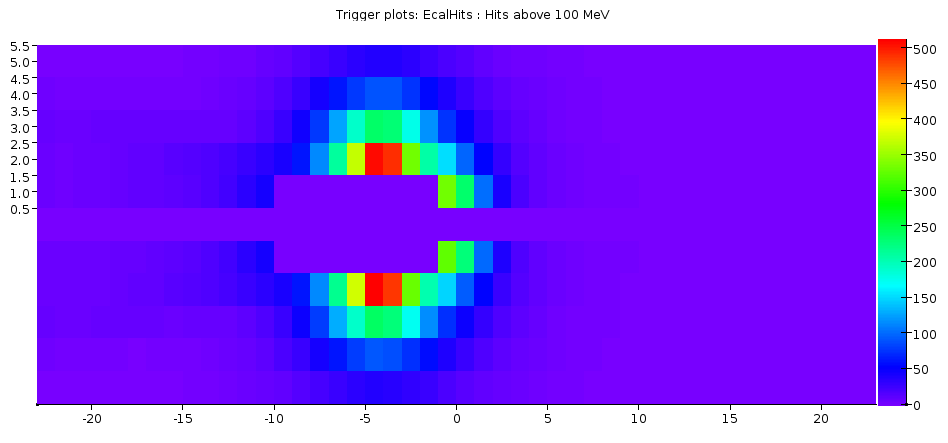
\includegraphics[width=0.7\textwidth]{performance/ecal_rate_100mev_22}

	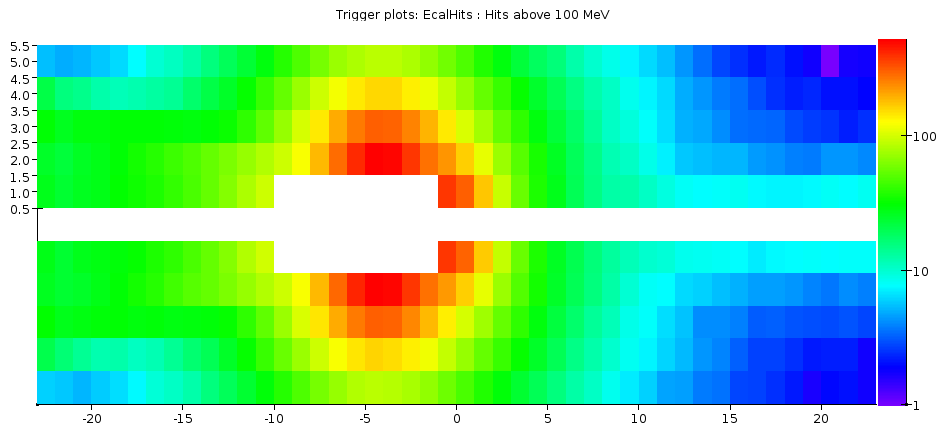
\includegraphics[width=0.7\textwidth]{performance/ecal_rate_100mev_22_log}
	\caption{\small{Rate of hits over 100 MeV (units of kHz) per crystal (X and Y axes are the crystal index), 
for 2.2 GeV beam at 200 nA. Top plot uses linear scale for the Z-axis; bottom plot is log scale.}}
	\label{fig:ecal_rate}
\end{figure}

\begin{figure}[ht]
	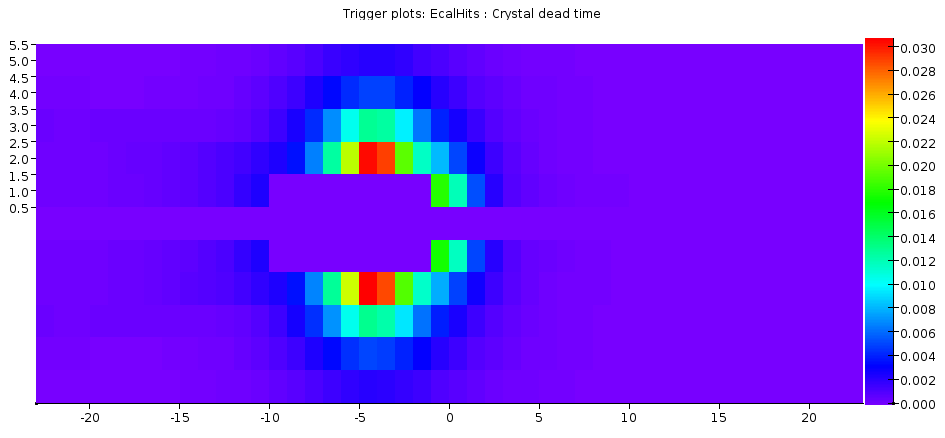
\includegraphics[width=0.7\textwidth]{performance/ecal_deadtime_22}
	\caption{\small{ECal readout deadtime fraction for 2.2 GeV beam at 200 nA, 
with a threshold of 75 MeV for each crystal.}}
	\label{fig:ecal_deadtime}
\end{figure}

\subsection{ECal trigger rates}
\label{sec:ecaltrigg}
%\subsubsection{ECal trigger performance}
The proposed ECal trigger was simulated to test trigger cuts, verify
that the trigger has acceptable efficiency for A' events, and verify 
that the trigger rate is compatible with the HPS DAQ in all running conditions. 

The CEBAF beam bunch structure was simulated by sending one bunch 
equivalent of electrons, 
625 (1.1 GeV), 2,500 (2.2 GeV) and 5,625 $e^-$'s (6.6 GeV), through 
the target, and total 50 million bunches of beam backgrounds 
(equivalent to 100 ms of beam) were 
generated at each beam energy. The details of the target interactions are given in Section \ref{sec:backgrounds}.
Since the trident production process 
was not in EGS5, trident events were generated with MadGraph/MadEvent 
and overlaid on the beam background bunches with average rate 
expected from the trident cross section.
For the trigger acceptance studies, A' events were generated with 
MadGraph/MadEvent at 1.1, 2.2, and 6.6 GeV.

The complete chain of signal evolution in the ECal crystals and 
signal processing through the trigger system was simulated
by following closely the ECal trigger description in Section \ref{sec:triggerdaq}. 
Starting from the energy deposits in the ECal crystals, signals were 
generated using the CR-RC shaper function with a time constant of 15 ns
measured with the ECal crystals, amplitudes were sampled and pulse data 
evaluated every 4 ns (simulating FADC), and the cluster 
finding algorithm and trigger logic were applied (simulating CTP and SSP). 
The simulation has been tested against the actual performance of the test run detector and DAQ: see Section \ref{sec:ecalperformance}.

The trigger parameters described in Section \ref{sec:triggerdaq} are 
chosen by running the simulation and plotting the relevant variables 
for beam background and A' events. This is done for each beam energy 
and a set of A' masses for each beam energy. 
Figure \ref{fig:coplanarity} shows the coplanarity angle vs. the azimuthal 
angle of the lower-energy cluster, indicating that A' events 
tend to have small coplanarity angles. Figure \ref{fig:energy-distance} shows
the distance from beam axis vs. energy of the lower-energy cluster,
indicating that the energy-distance cut can reduce the beam background effectively.
Figure \ref{fig:ediff} shows the cluster energy difference vs. energy sum,
indicating that the energy sum cut can retain A' events effectively.       


These cuts are chosen to lie between the loosest reasonable values (accept as many A' events as possible) and the tightest (reject as many background events as possible). In some cases this leads to different cut values at different beam energies---for example, the coplanarity cut is looser at 1.1 GeV because the background events are clustered at large uncoplanarity and a relatively loose cut rejects most of them, but the cut is tighter at higher beam energies.

\begin{figure}[ht]
	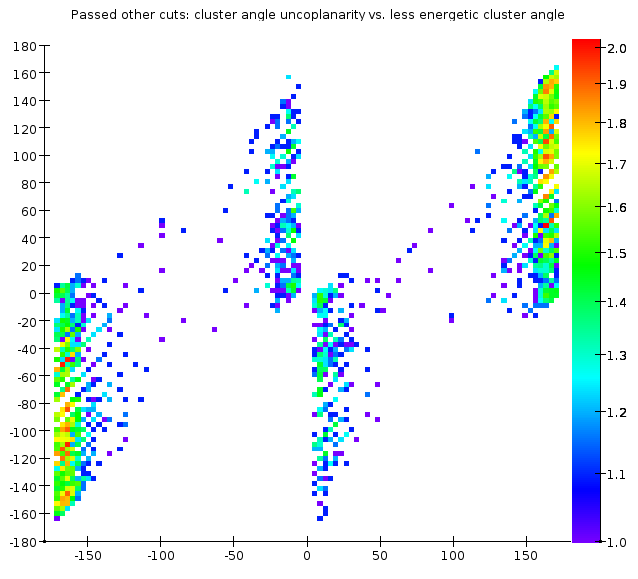
\includegraphics[width=0.4\textwidth]{performance/trigger/coplanarity_22}
	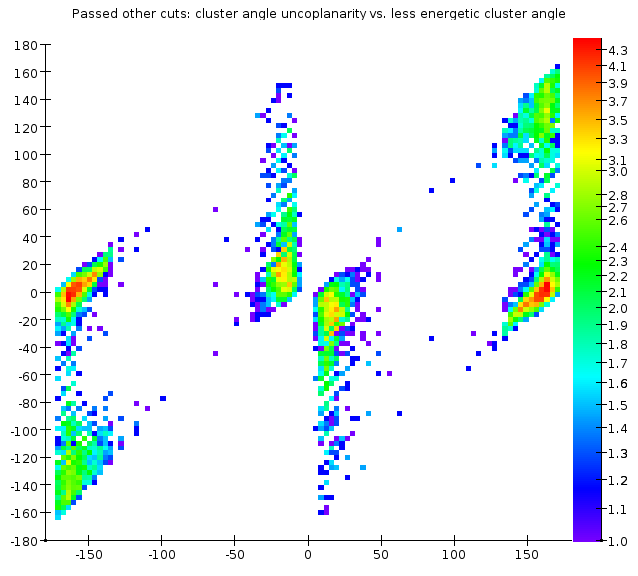
\includegraphics[width=0.4\textwidth]{performance/trigger/coplanarity_22_075mev}
	\caption{\small{Deviation of cluster pairs from coplanarity (units of degrees) for 2.2 GeV beam; background and 75 MeV A' tridents are shown. The X-axis is the azimuth around the beam axis ($\phi_1$) of the lower-energy cluster, such that 0 degrees is the positron side of the detector and 180 degrees is the electron side; the Y-axis is the difference between the azimuth angles ($\phi_1-\phi_2 - 180$) of the two clusters. The coplanarity cut's acceptance region is the space between the red lines.}}
	\label{fig:coplanarity}
\end{figure}

\begin{figure}[ht]
	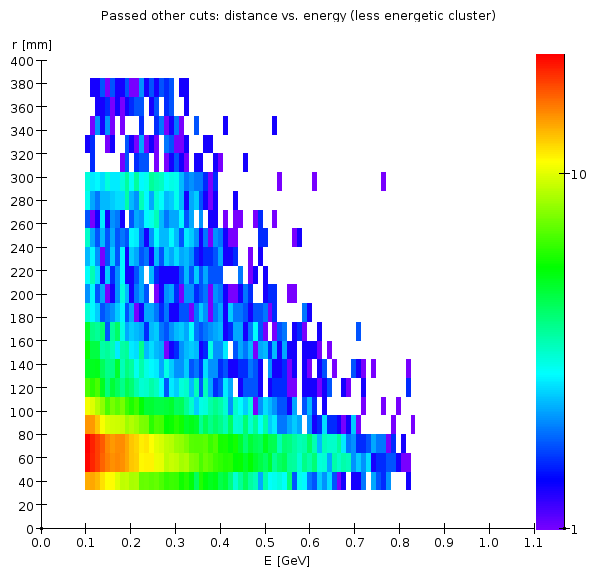
\includegraphics[width=0.4\textwidth]{performance/trigger/energy-distance_22}
	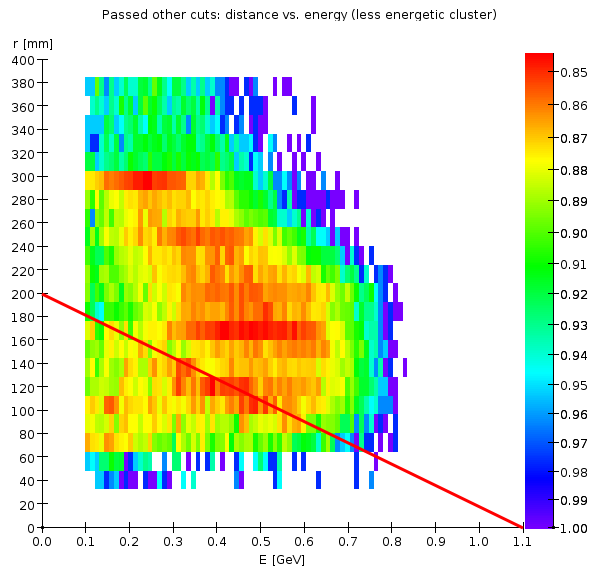
\includegraphics[width=0.4\textwidth]{performance/trigger/energy-distance_22_075mev}
	\caption{\small{Energy and distance from beam axis of the lower-energy cluster, for 2.2 GeV beam; background and 75 MeV A' tridents are shown. The energy-distance cut's acceptance region is above the red line.}}
	\label{fig:energy-distance}
\end{figure}

\begin{figure}[ht]
	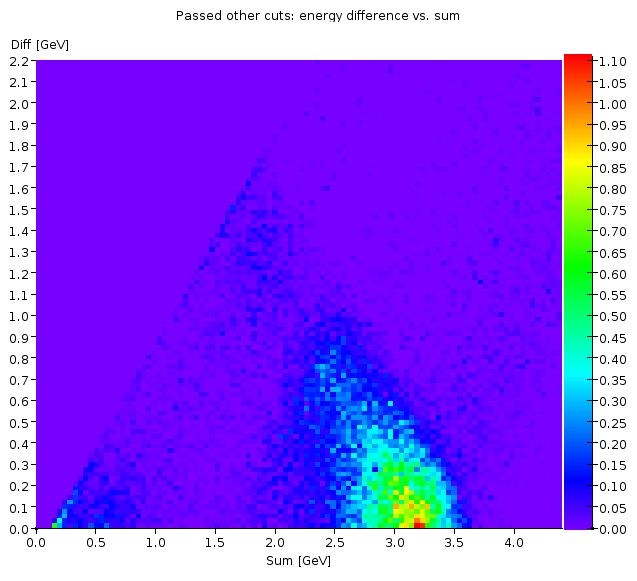
\includegraphics[width=0.4\textwidth]{performance/trigger/ediff_22}
	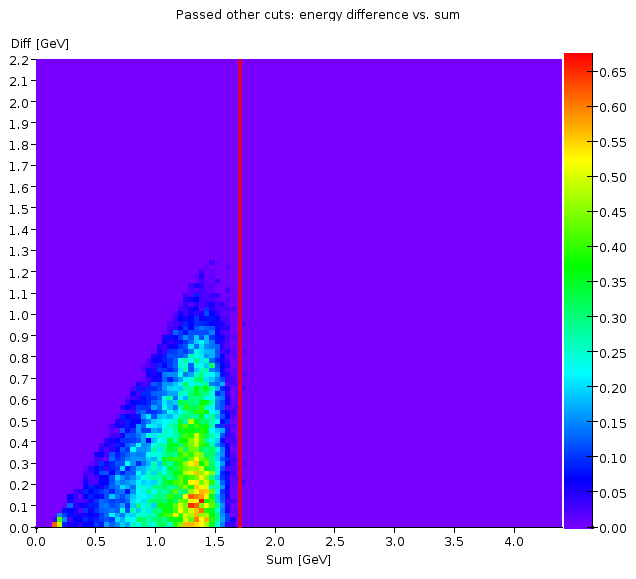
\includegraphics[width=0.4\textwidth]{performance/trigger/ediff_22_075mev}
	\caption{\small{Energy sum and difference of cluster pairs, for 2.2 GeV beam; background and 75 MeV A' tridents are shown. The energy difference cut's acceptance region is left of the red line.}}
	\label{fig:ediff}
\end{figure}

The following trigger parameters were determined to be independent of beam energy:
\begin{itemize}
	\item Minimum cluster energy ($E_{min}$): 0.1 GeV
	\item Distance ($r_{edist}$) in the energy-distance cut: 200 mm
	\item Energy ($E_{edist}$) in the energy-distance cut: $0.5\times E_{beam}$
\end{itemize}

Table \ref{tab:trigcuts} summarizes the trigger parameters that were found dependent on the beam energy. 
The remaining trigger parameters given in Section \ref{sec:triggerdaq} did not have a significant 
effect on specificity of the trigger.

\begin{table}
	\begin{tabular}{|l|r|r|r|}
		\hline
		Beam energy [GeV] & $E_{max}$ [GeV] & $Esum_{max}$ [GeV] & $\Delta\phi_{max}$ [$^\circ$] \\
		\hline
		1.1	&	0.7	&	0.8	&	90\\
		2.2	&	1.6	&	1.7	&	45\\
		6.6	&	5.0	&	5.5	&	60\\
		\hline
	\end{tabular}
	\caption{ {\small Trigger parameters optimized for different beam energies.}
	\label{tab:trigcuts}}
\end{table}

Trigger rates are shown in Table \ref{tab:trigrates}. These rates are safely under the maximum readout rate of 43 kHz set by the SVT DAQ. 
Furthermore, tightening the coplanarity and energy-distance cuts lowers trigger rates to $\approx 10$ kHz at 1.1 and 2.2 GeV and $\approx 5$ kHz at 6.6 GeV, while reducing the A' efficiency by no more than 2 percentage points; this provides further safety margin in case trigger or data rates are higher than expected.
The addition of pions to the 6.6 GeV background sample has only a small effect on the trigger rate.

\begin{table}
	\begin{tabular}{|l|r|}
		\hline
		Sample &  Rate (kHz)\\
		\hline
		1.1 GeV	beam background 				& 15.7 $\pm$ 0.4	\\
		1.1 GeV beam background+tridents			& 18.3 $\pm$ 0.4	\\
		2.2 GeV	beam background 				& 11.2 $\pm$ 0.3	\\
		2.2 GeV beam background+tridents			& 15.8 $\pm$ 0.4	\\
		6.6 GeV	beam background 				& 10.2 $\pm$ 0.3	\\
		6.6 GeV beam background+tridents			& 12.6 $\pm$ 0.4	\\
		6.6 GeV beam background+tridents+pions (FLUKA)	& 13.4 $\pm$ 0.4	\\
		6.6 GeV beam background+tridents+pions (G4)	& 13.5 $\pm$ 0.4	\\
		\hline
	\end{tabular}
	\caption{ {\small Trigger rates using various background samples, with statistical uncertainties. }
	\label{tab:trigrates}}
\end{table}

Trigger efficiency for A' events is defined as the fraction of A' tridents (generated without fiducial cuts) that produce a trigger.

For the performance of the experiment, we are interested in the combined efficiency of the trigger and tracker: the fraction of A' tridents that produce a trigger and leave enough hits in the tracker for a pair of tracks to be reconstructed.
We simulate charge deposition and readout of the tracker (turning off the generation of noise hits), and check each sensor for hits. 
If the DAQ reads out hits in four stereo pairs in each half of the tracker, the event is in the combined acceptance.

Figure \ref{fig:trigeff} shows the ECal trigger efficiency and the ECal/SVT-combined efficiencies for A' events at 1.1, 2.2, and 6.6 GeV. 
Both trigger and tracker acceptances are dominated by the geometric acceptances of the ECal and tracker.
A' prompt decays are assumed.

\begin{figure}[ht]
	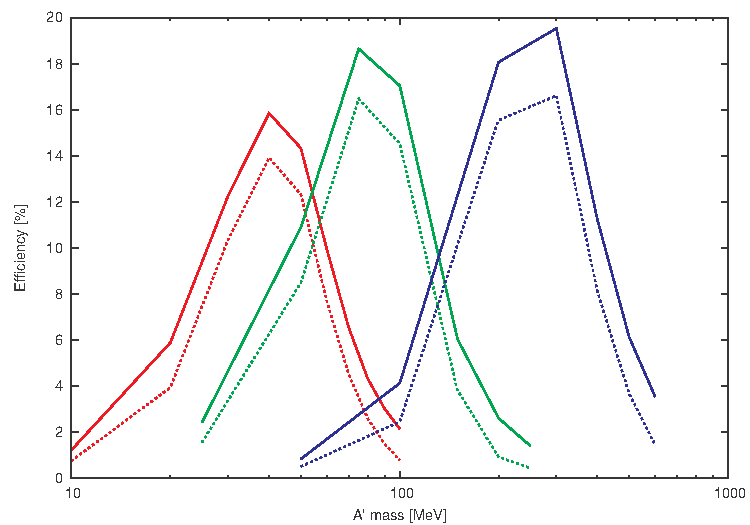
\includegraphics[width=\textwidth]{performance/trigger/ap_eff}
	\caption{\small{Trigger efficiency (solid lines) and combined efficiency (dashed lines) as a function of A' mass, at beam energies of 1.1, 2.2 and 6.6 GeV (red, green and blue respectively).}}
	\label{fig:trigeff}
\end{figure}



\subsubsection{Muon system trigger rates}
\label{sec:muontrigg}

Like the ECal, the muon system trigger rates are dominated by beam backgrounds.  
A GEANT4 model of the HPS detector was used to estimate the rates, following the conceptual design for the muon system presented in 
Section\ref{sec:muon}. Figure \ref{fig:HPS_view2} shows the layout of the system. Each of eight hodoscope layers (four layers in 
the top part of the detector and four in the bottom) consists of two planes of scintillator strips. One plane, called the Y-plane, has strips 
oriented horizontally. The other, called the X-plane, has them oriented vertically. The Y-strips are segmented exactly in the middle
and outside ends, left or right, are read out. 
Six Y-strips make up each half plane, so the total number of Y-strips is 48. 
X-planes are divided into 4.5 cm wide segments, with 240 strips in total. It should be noted that the number of vertical strips 
in the conceptual design is only 208 to limit the total number of readout channels to 256, one crate's worth. Since the rates in the 
vertical strips at the edges of the hodoscope are very low, eight strips in each 
plane can be paired to make four readout channels without negatively impacting the detector occupancy. In Table \ref{tb:muonstrp}, 
the lengths and widths of the detector readout segments (counters) used in the simulation are presented. There is a $14$ cm wide 
and $3.5$ cm high gap 
introduced into the model, centered on the point where the electron beam passes through the muon vacuum chamber, to avoid the high rate region.
As shown in Figure \ref{fig:xymu} 
this gap has a negligible effect on the detection efficiency of muon pairs from $\ap$ decays. 

\begin{table}[htdp]
\caption{Lengths and widths of the hodoscope strips. Dimensions are centimeters.}
\begin{center}
\begin{tabular}{|c|c|c|c|c|}
\hline\hline
Readout plane& Layer 1&Layer 2&Layer 3& Layer 4 \\
\hline
X-plane width& 4.5& 4.5 & 4.5 & 4.5  \\
X-plane length&10.5&11.5&12.5&13.5\\
\hline
Y-plane width& 3.5 all three&3.5, 4, 4  & 3.5, 4.5, 4.5 & 4.5 all three\\
Y-plane length&56&62.5&70&76\\
\hline\hline
\end{tabular}
\end{center}
\label{tb:muonstrp}
\end{table}%

Events generated in EGS5 were used as an input to the GEANT4 simulation. The CEBAF beam bunch structure was simulated by sending 
one bunch equivalent of electrons, 5,625 $e^-$'s (6.6 GeV), through 
the target to generate secondaries and scattered beam particles. The secondaries were followed through the apparatus
to simulate the detector response. As expected, the 
highest background rates are seen in the Layer 1 hodoscope and are $\sim 0.7$ MHz in both the X-strips near the electron beam location and 
the beam-left Y-strip closest to the beam plane, see Figure \ref{fig:l1rates}. Rates in the vertical strips far from the 
beam position are very low, allowing multiple strips to be combined into a single readout channel in order to reduce the number 
of PMTs and electronic channels.  

\begin{figure}[htbp]
\begin{center}
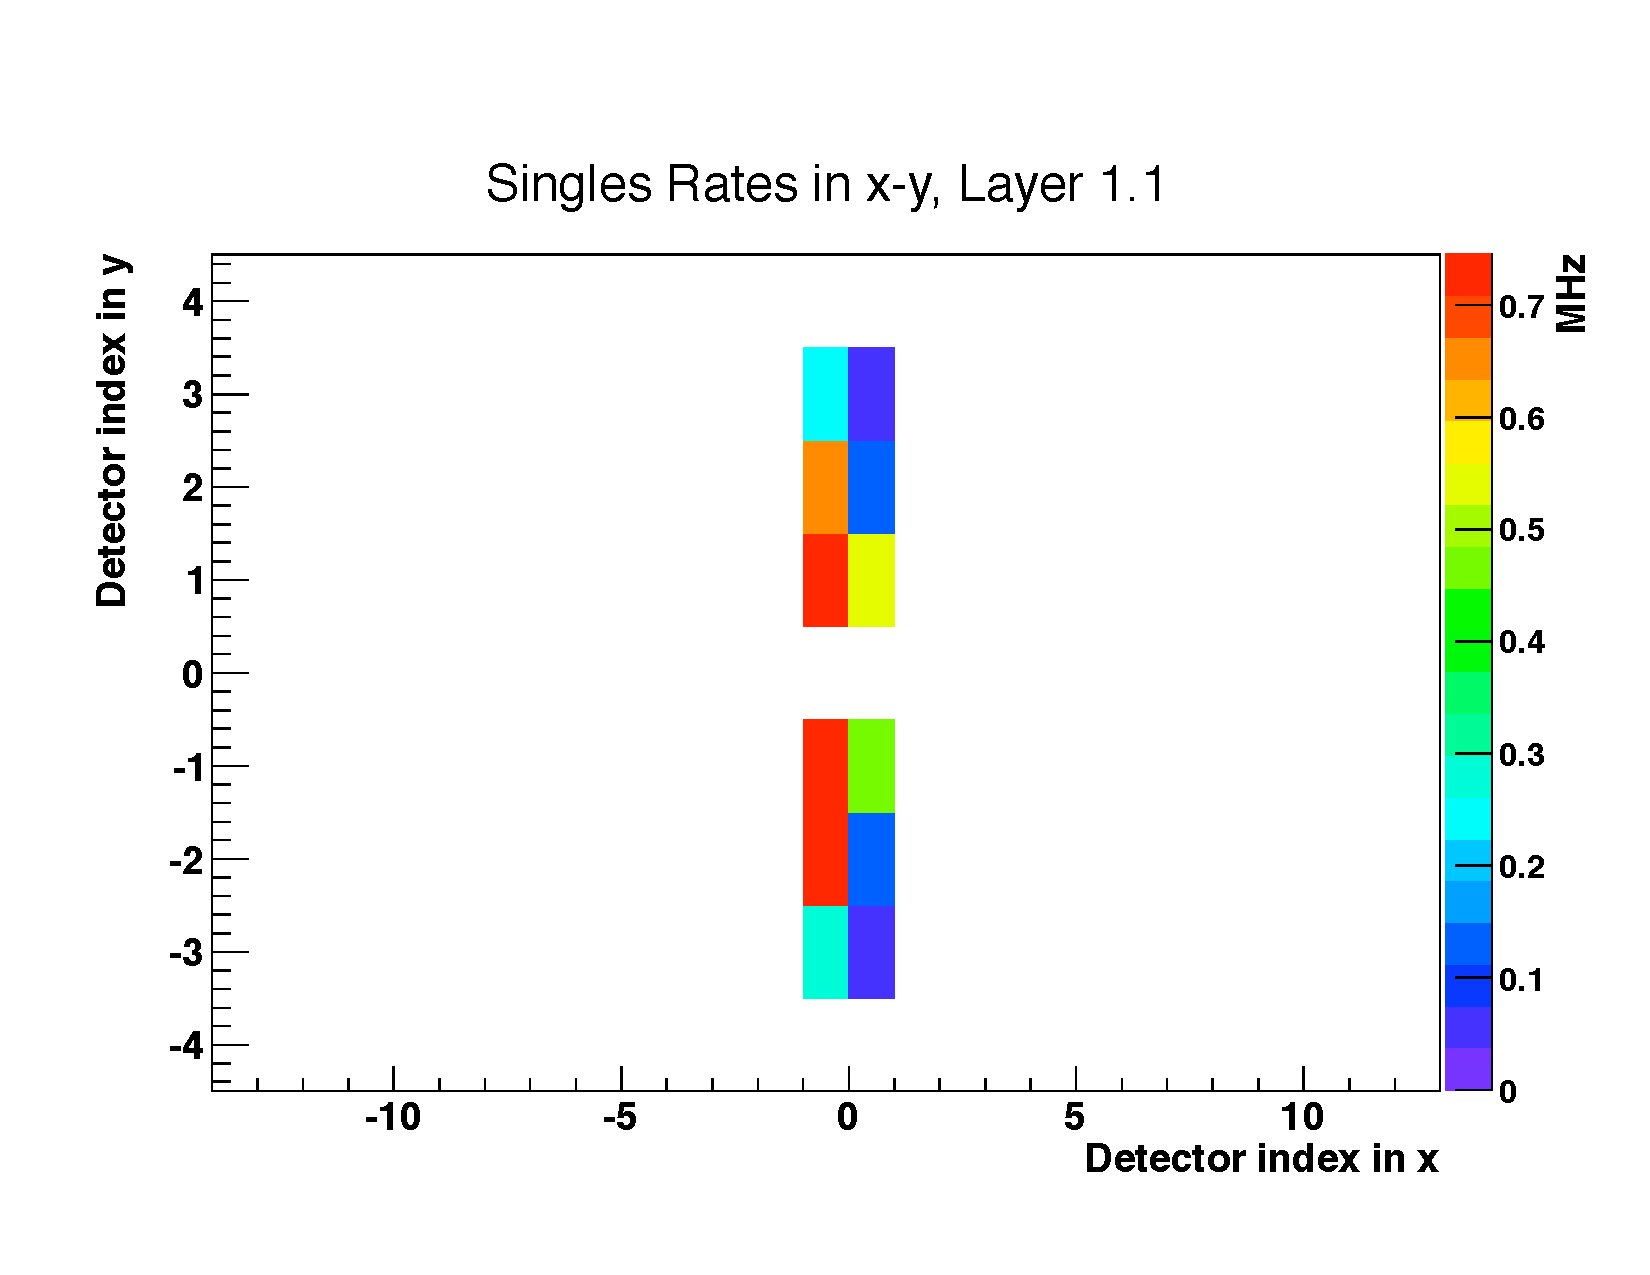
\includegraphics[width=0.475\textwidth]{performance/trigger/muon_singles1}
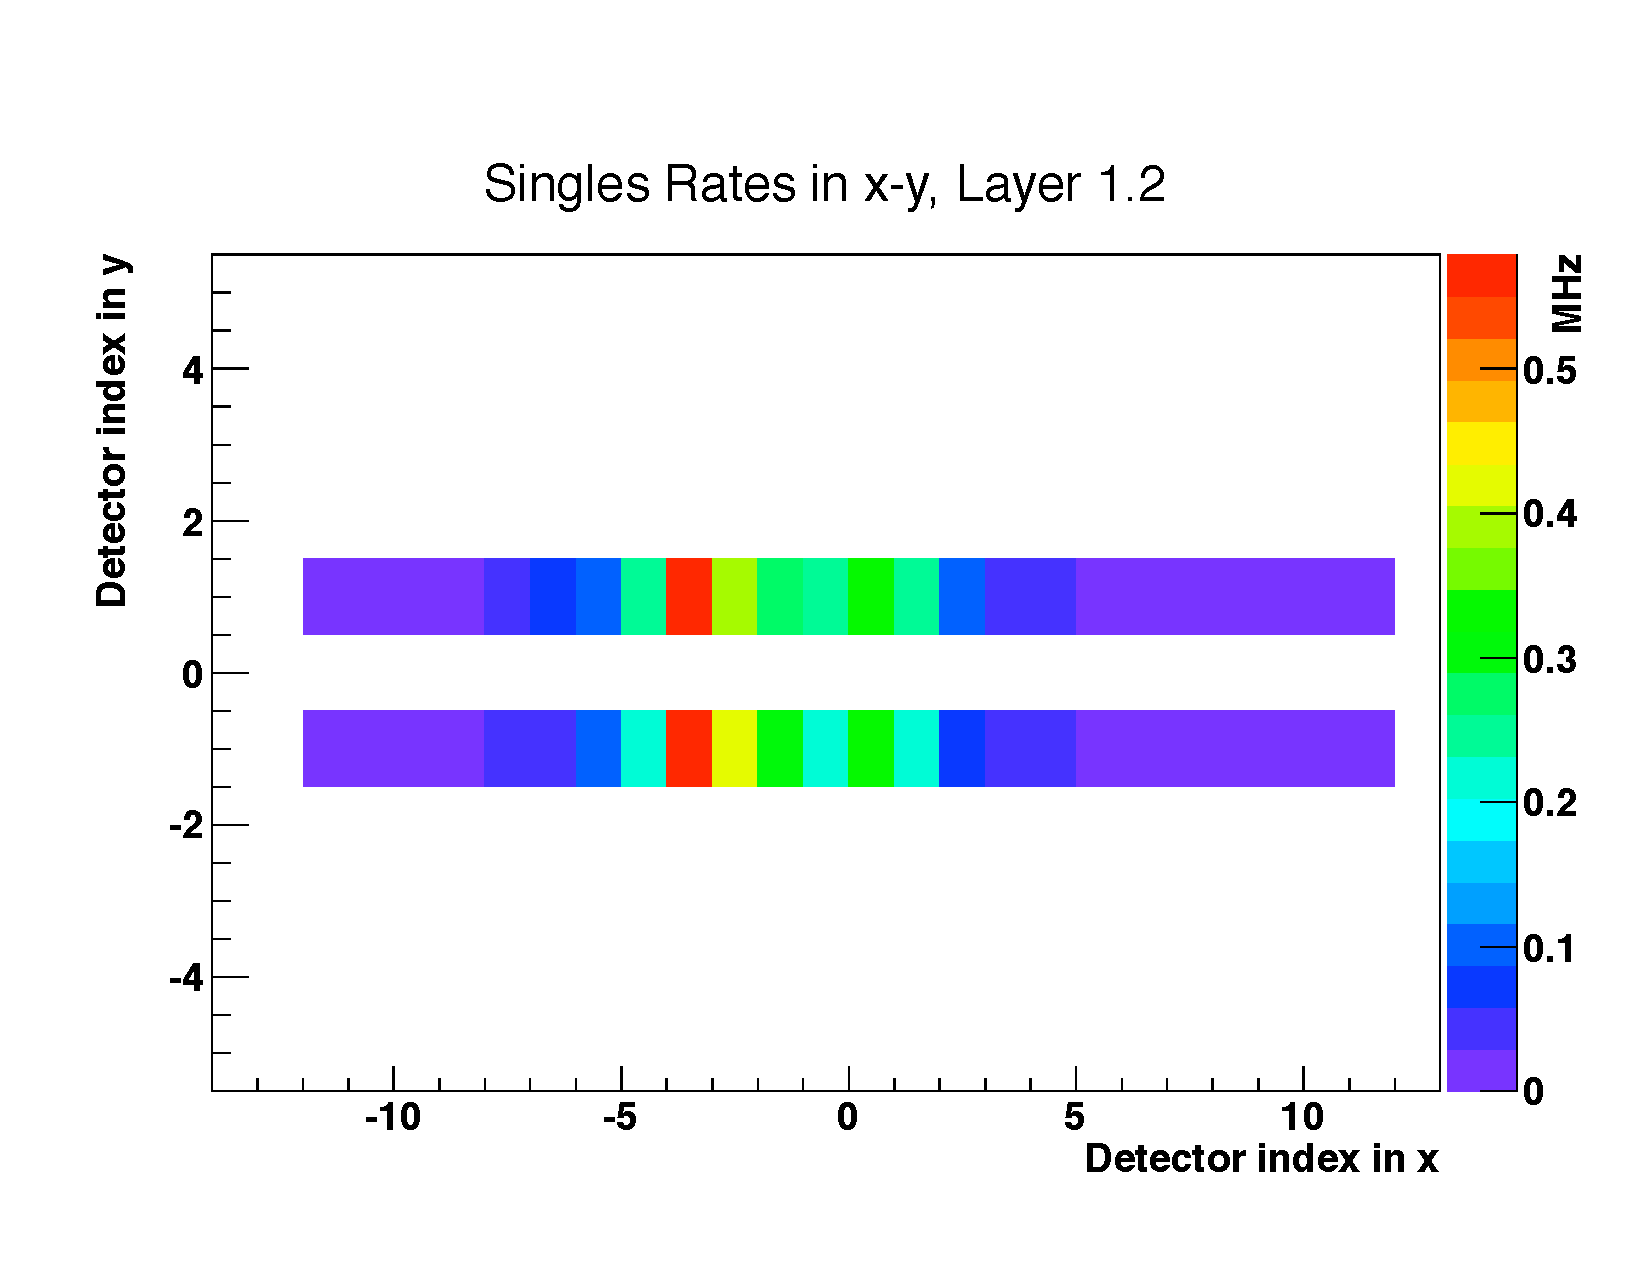
\includegraphics[width=0.475\textwidth]{performance/trigger/muon_singles2}
\caption{Rates in Y- (left) and X-planes (right) of the Layer 1 hodoscopes for hits with energy deposition $> 0.5$ MeV.}
\label{fig:l1rates}
\end{center}
\end{figure}

The coincidence rates between hodoscope planes in a given layer and between different layers have been studied using a $16$ ns coincidence 
time window. 
On the left of  Figure \ref{fig:c1rates}, the coincidence rates between X- and Y-quadrants, top-left (TL), top-right (TR), bottom-left 
(BL), and bottom-right (BR) of the Layer 1 hodoscope are shown. On the right, the figure shows coincidence rates of respective 
quadrants of Layers 1 and 2. The fact that there is a significant reduction of the rates from 2-plane (~1.2 MHz) to 2-layers (0.07MHz) 
coincidences indicates that hits are mostly from uncorrelated background. For the muon trigger, a coincidence of two opposite quadrants 
(TLxBR) or (TRxBL) is required along with triple coincidences of the first three layers of hodoscopes in each quadrant. The rates of the 
triple quadrant  
coincidences within $16$ ns are shown in Figure \ref{fig:c3rates}. The maximum trigger rates are in the beam-right (electron side) 
quadrants and are on order of $7$ kHz. In the beam-left quadrants (positron side), the tripple coincidence rates are $<1$ kHz. 
Since an overall trigger requires hits in two opposite quandrants, the maximum 
rate will be $<1$ kHz. While a further reduction of rates will be possible with the inclusion of 
MIP hits in the ECal, the $<1$ kHz is a small addition to the total trigger rate from the Ecal trigger (see discussions in 
Section \ref{sec:ecaltrigg}) and will keep overall trigger rate well within the limit of allowed rates for the HPS DAQ.   

\begin{figure}[htbp]
\begin{center}
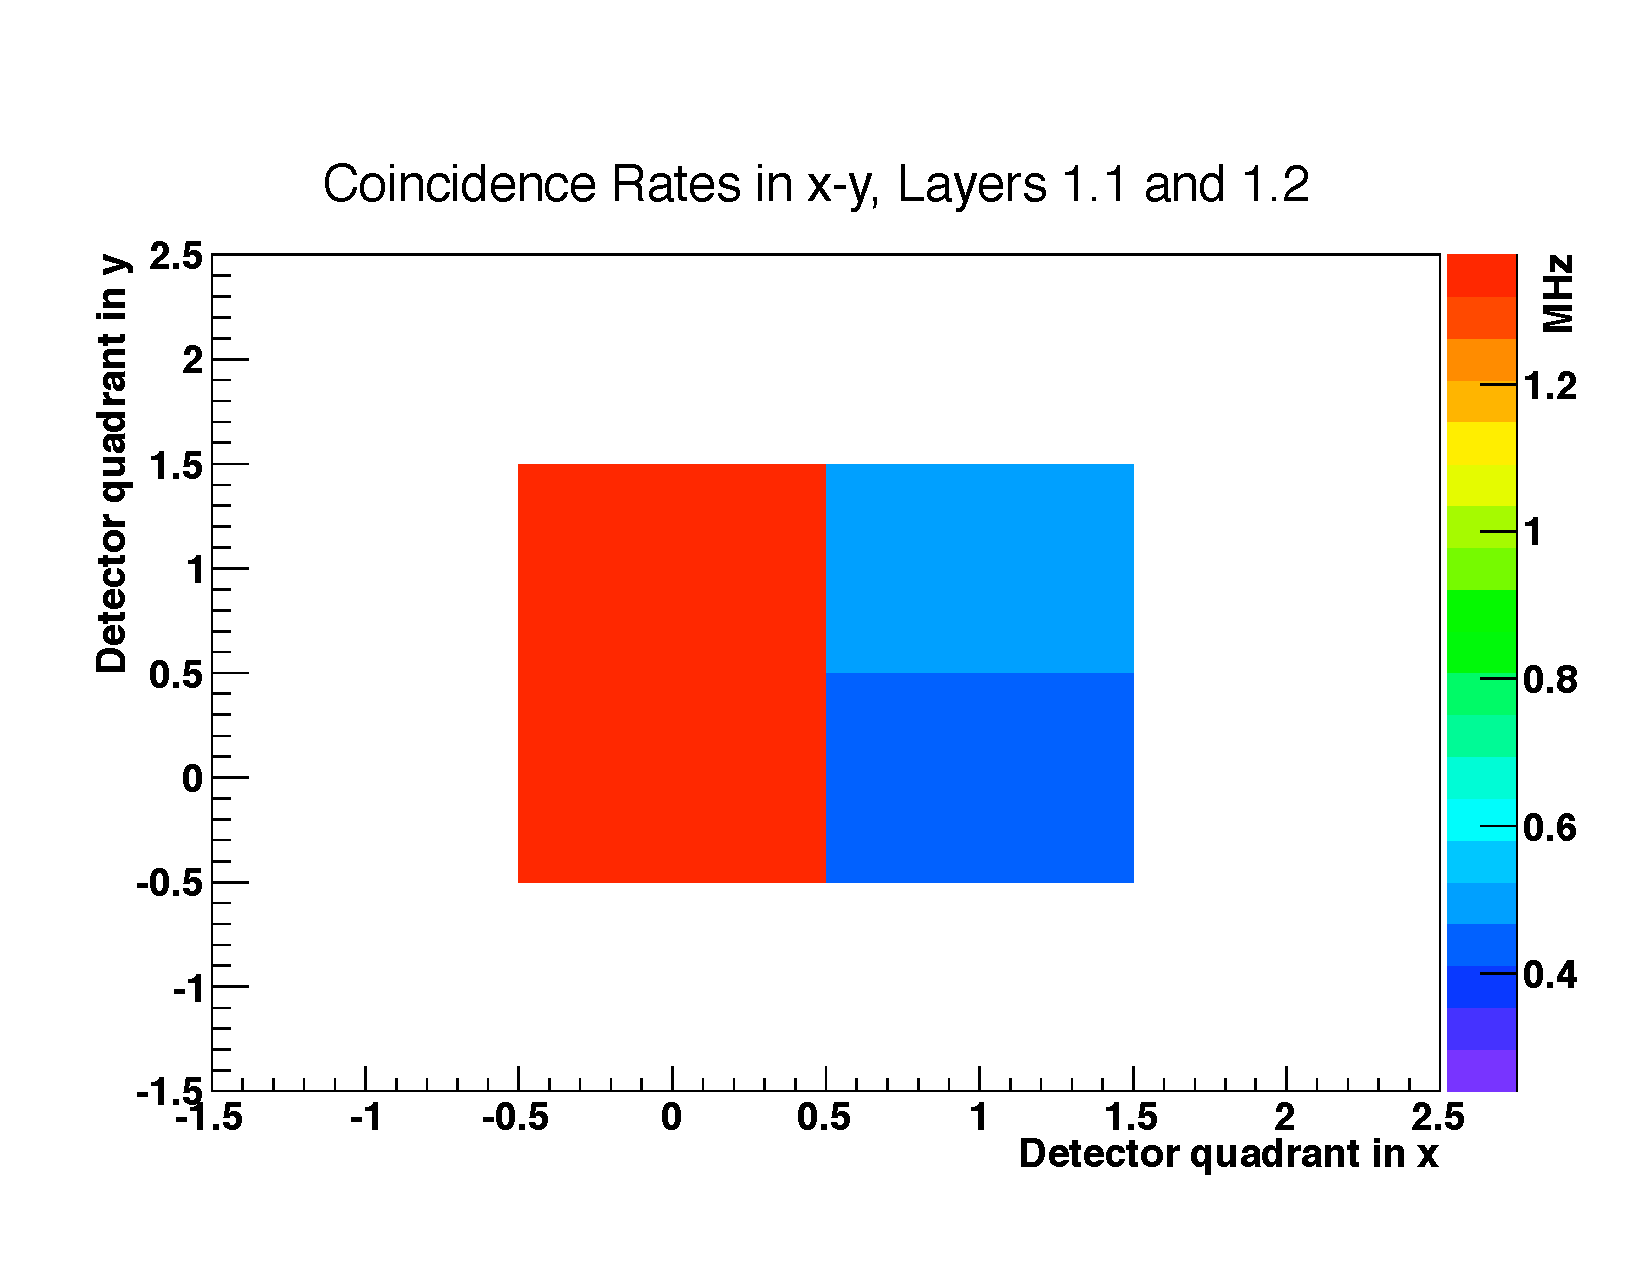
\includegraphics[width=0.475\textwidth]{performance/trigger/muon_coinrate1}
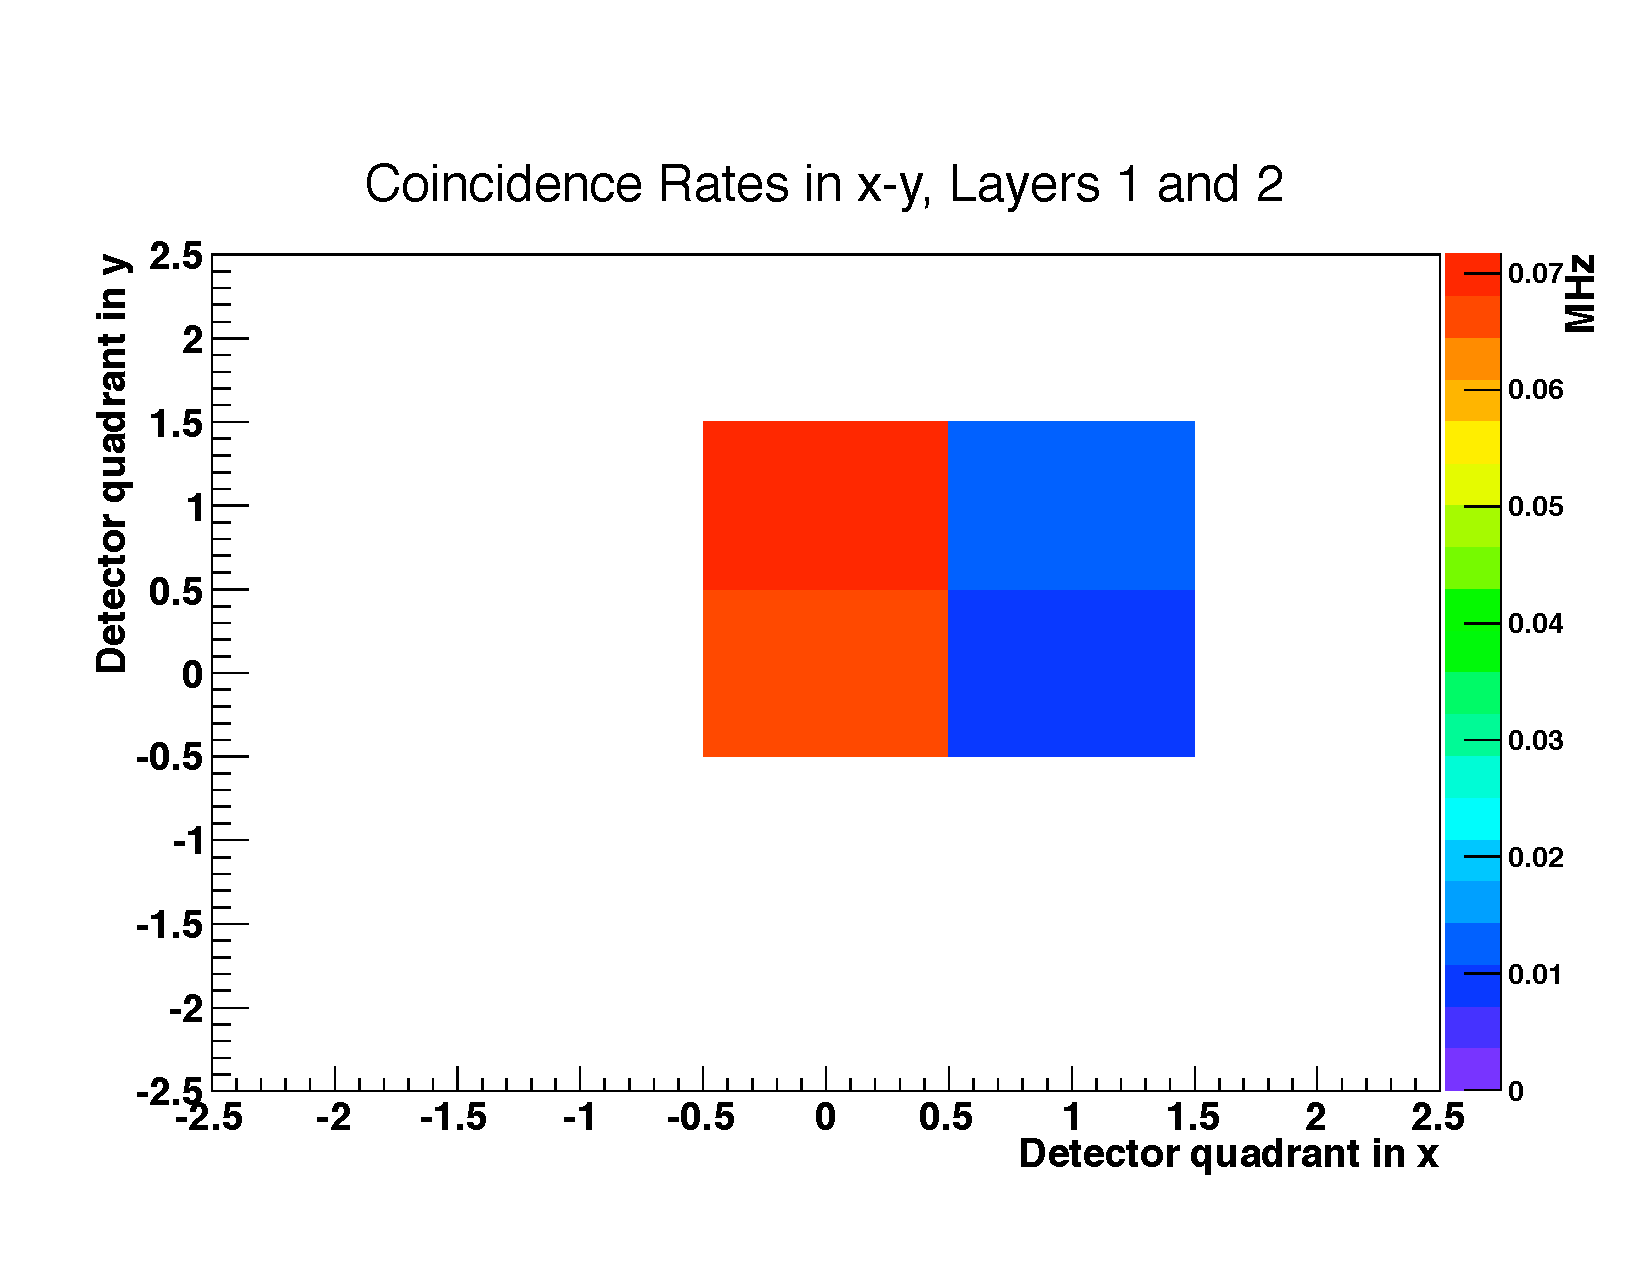
\includegraphics[width=0.475\textwidth]{performance/trigger/muon_coinrate2}
\caption{Coincidence rates between X- and Y-quadrants of the Layer 1 hodoscope (left graph) and coincidence rates between Layer 1 and 2 
(right graph). }
\label{fig:c1rates}
\end{center}
\end{figure}

\begin{figure}[htbp]
\begin{center}
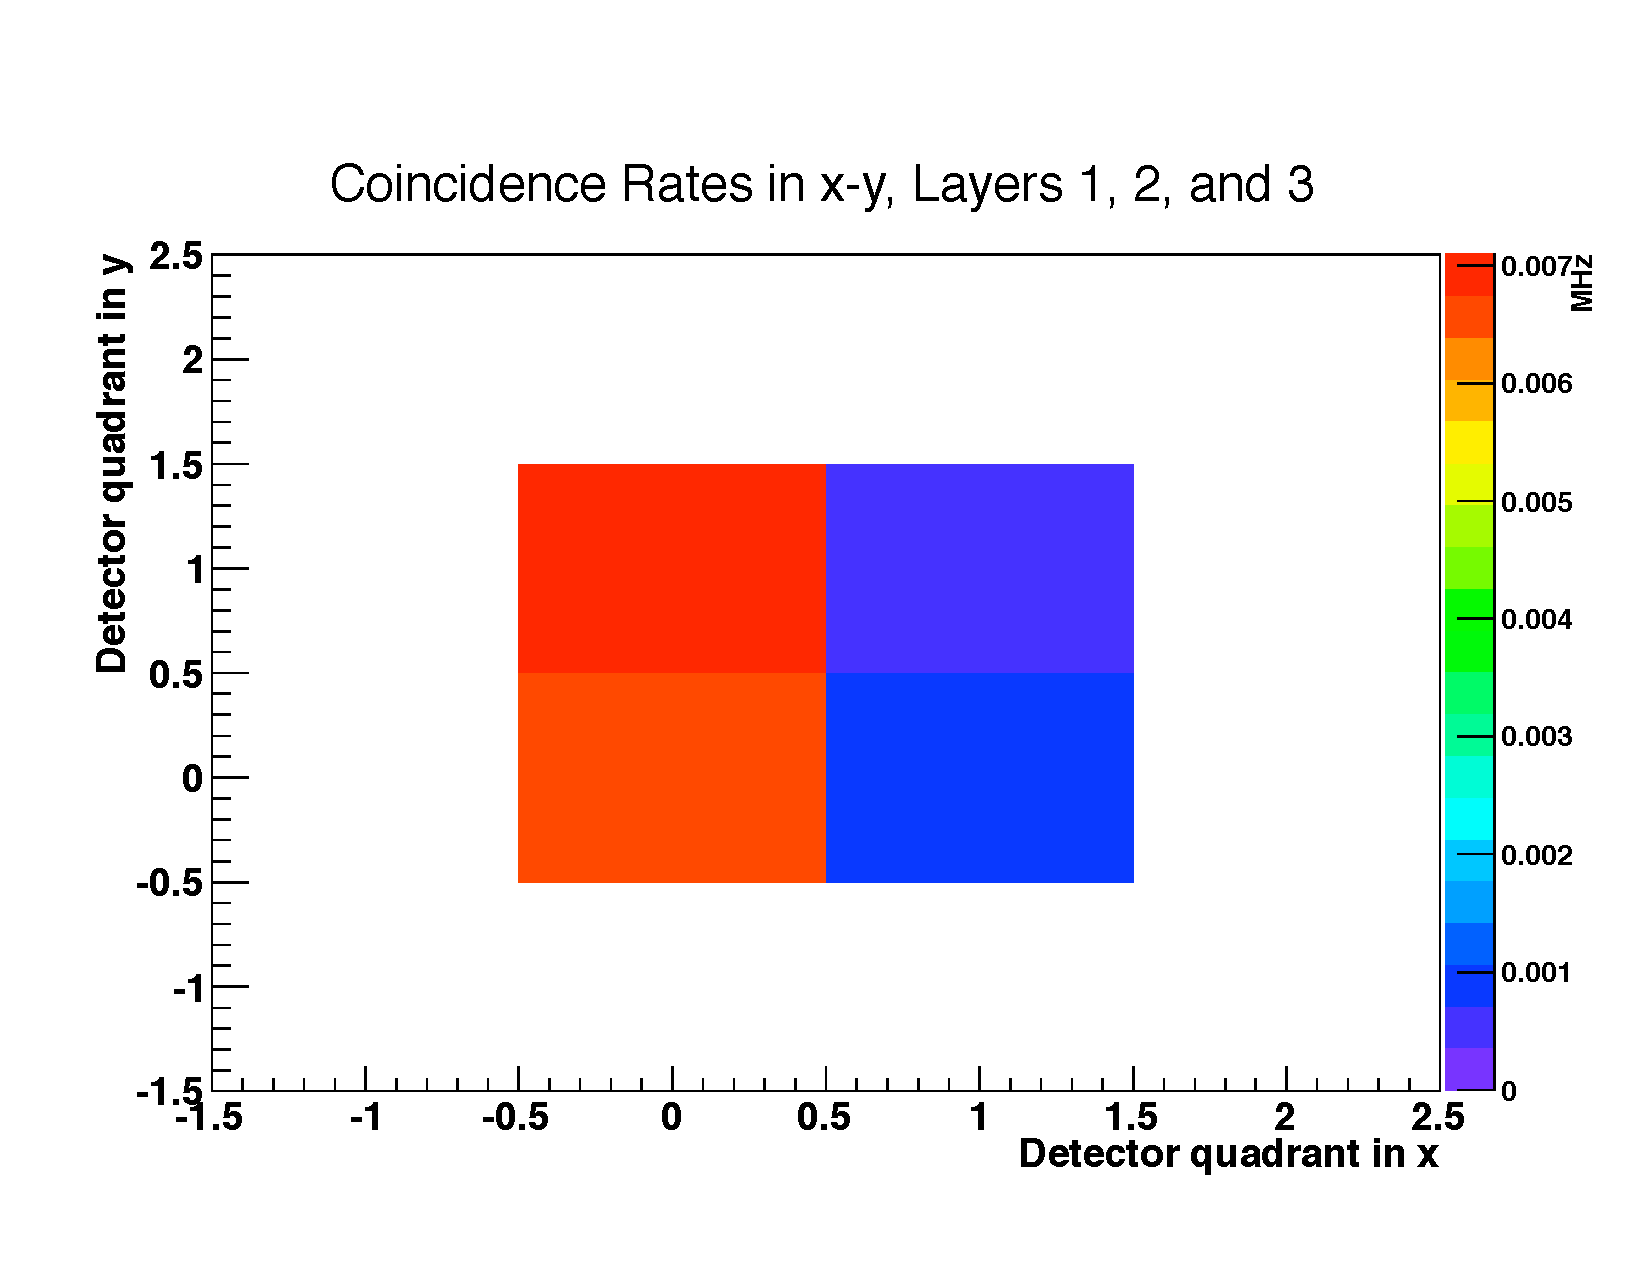
\includegraphics[width=\textwidth]{performance/trigger/muon_coinrate3}
\caption{Coincidence rates in first three layers of muon hodoscopes. The coincidence time window is set to $16$ ns. }
\label{fig:c3rates}
\end{center}
\end{figure}







%\subsubsection{Muon trigger performance}

\subsection{Track reconstruction}
\label{sec:trkperf}


In order to study the tracking performance of the detector, we use samples of $A'$ events 
at a variety of energies and decay lengths.  On top of each event, we overlay backgrounds 
produced by the passage of  beam electrons equivalent to our optimized run conditions at
different beam energies and with a W target and a beamspot of Gaussian sigma of 40$\mu$m in the vertical direction and 
200$\mu$m in the horizontal. The beam energies, currents, target thickness and analyzing magnetic field  used for these simulations are:
\begin{itemize}
\item 50nA at 1.1 GeV with $X_0=0.125$\% and  B=0.25 T
\item 200nA at 2.2 GeV with $X_0=0.125$\% and  B=0.5 T
\item 300nA at 4.4 GeV with $X_0=0.25$\% and  B=1.0 T
\item 450nA at 6.6 GeV with $X_0=0.25$\% and  B=1.5 T
\end{itemize}
At each energy, we evaluate momentum, invariant mass, and vertex resolution.  The plots shown in the following section typically use the 4.4 GeV beam as an example.  

\subsection{Tracking Efficiency, Pattern Recognition and Fake Rates}

Due to the requirements imposed on the tracks, the efficiency for finding tracks in the 
geometric acceptance is not 1. The average track reconstruction efficiency is 98\% (Figure \ref{fig:trkeff}) and 
the bulk of the inefficiency comes from the cut on the total $\chi^2$ of the track. 
Of the reconstructed tracks, a small percentage include a hit that is not from 
the correct electron.  These ``bad'' hits may be from one of the high energy beam 
electrons scattered from the target into the detector or from a lower energy secondary.  
The left plot of Figure \ref{fig:badhits} shows the number of bad hits/track for both the electron 
and positron from the A' decay.  The number of tracks with 0 bad hits is $>$ 98\%.
% and 
%the positrons are slightly cleaner since occupancy of the positron side of the detector 
%is smaller.  
The right plot of Figure \ref{fig:badhits} shows the layer number of the bad hit.  
The rate of mishits are slightly higher in the downstream 3 modules due to the larger stereo angle % and are larger for positrons because they dip into the dead zone???%.  
We'll show how these bad hits affect the track parameters in the next section.


\begin{figure}
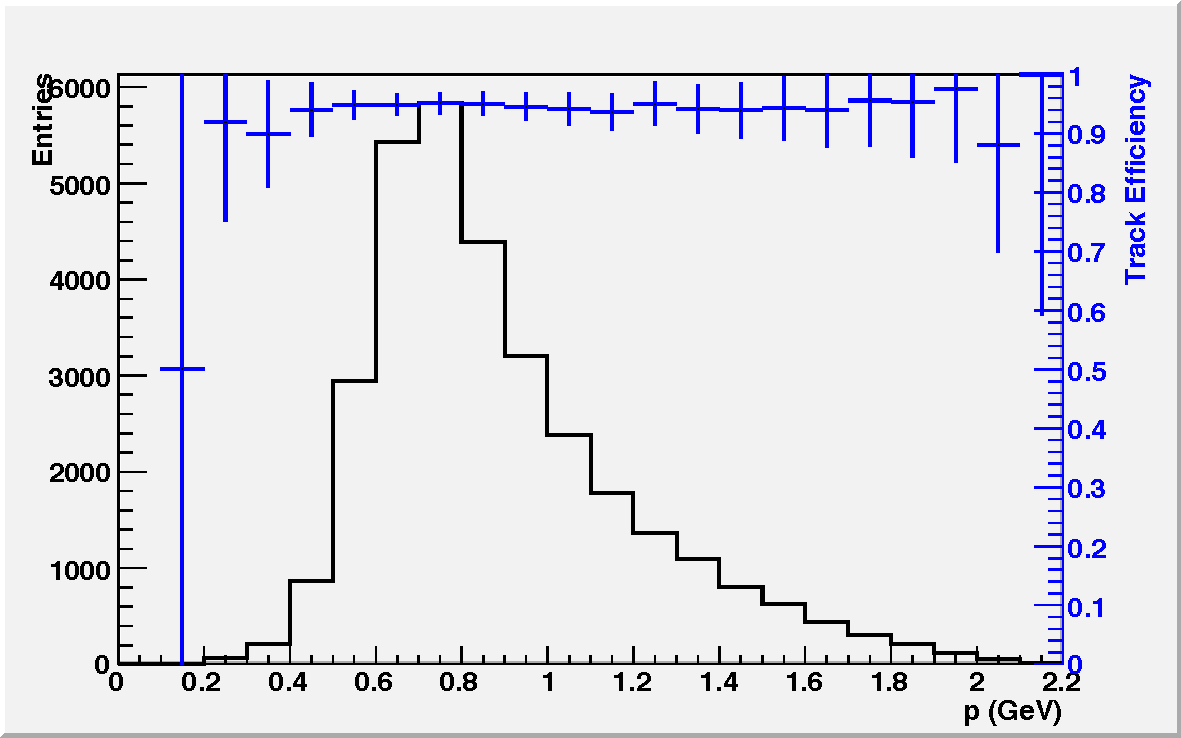
\includegraphics[scale=0.8]{performance/tracking_performance/pzE-Effic.pdf}
\caption{ Track reconstruction efficiency versus track momentum.  The blue histogram (right axis) show the track momentum distribution.  }
\label{fig:trkeffic}
\end{figure}

\begin{figure}
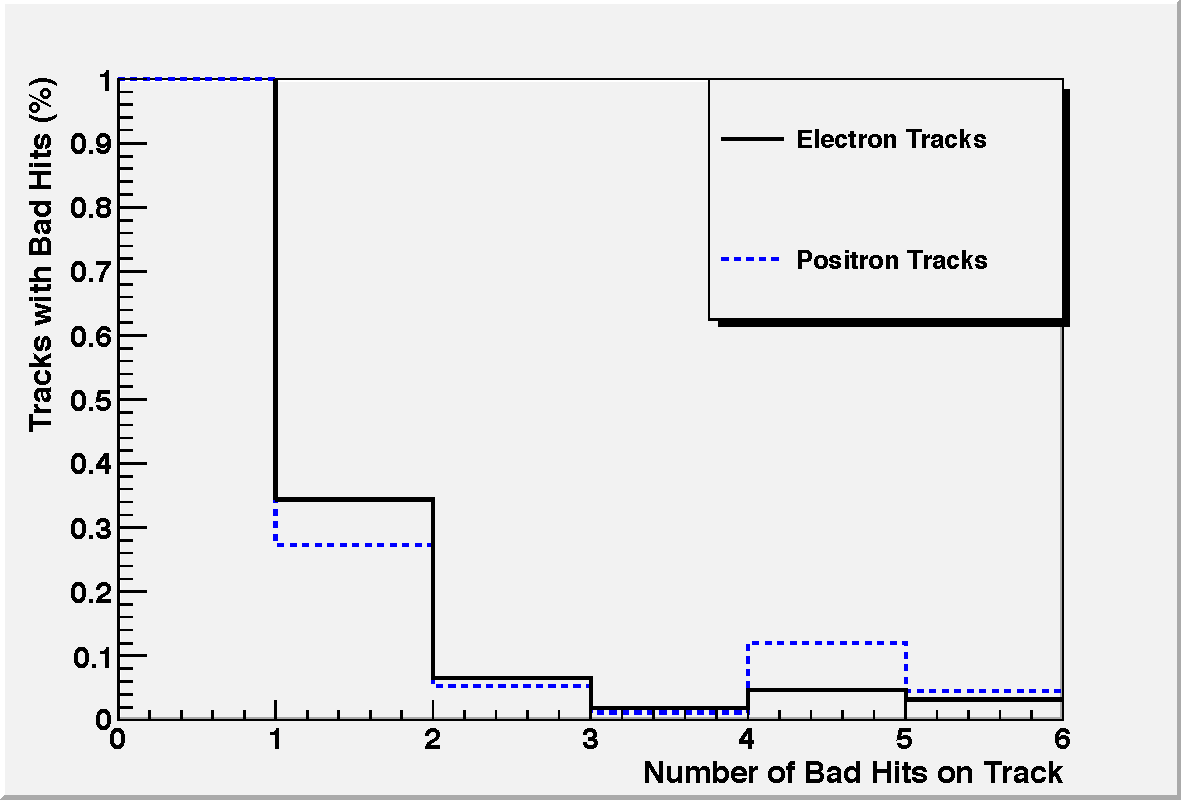
\includegraphics[scale=0.4]{performance/tracking_performance/nBadHits.pdf}
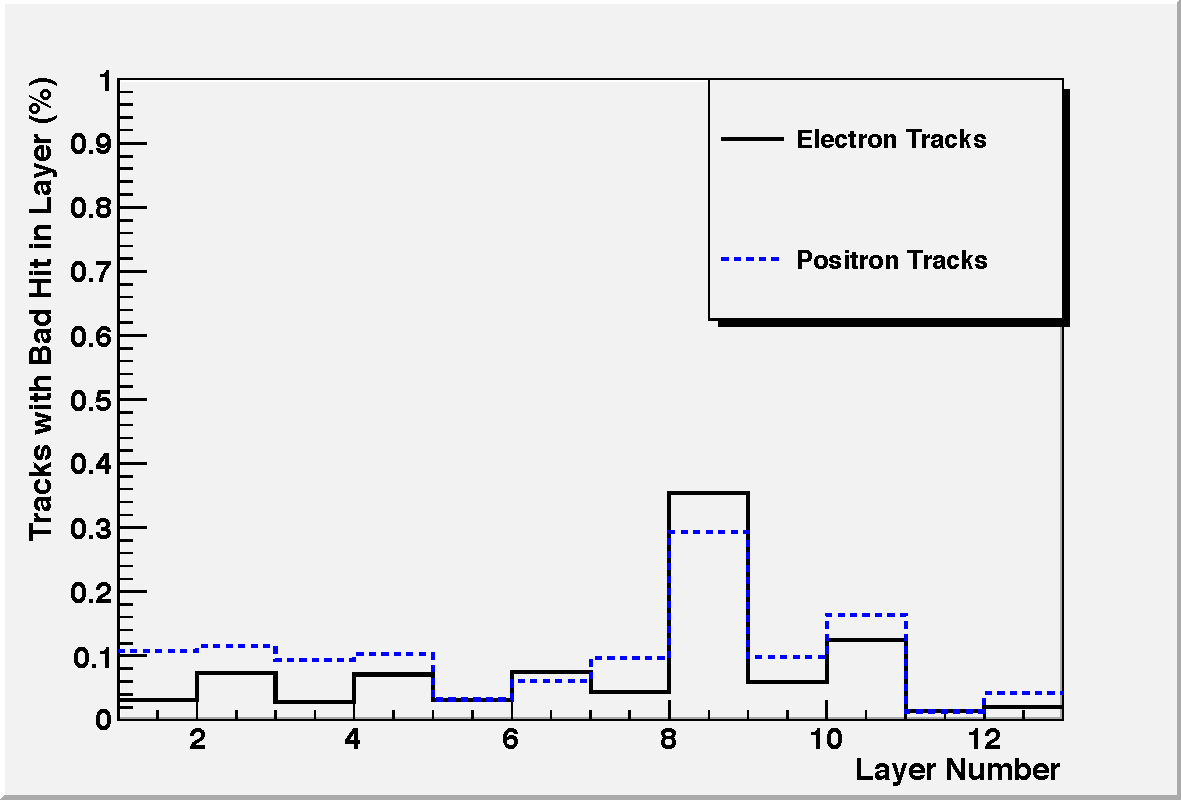
\includegraphics[scale=0.4]{performance/tracking_performance/BadLayer.pdf}
\caption{ The number of bad hits (left) and the layer number of the bad hit (right) 
for electron (black) and positron (blue) tracks.   }
\label{fig:badhits}
\end{figure}


\subsection{Track Momentum and Spatial Resolution}

The momentum resolution is shown in Figure \ref{fig:trkmom} as a function of momentum for tracks with 
0 bad hits and for tracks with one or more.  The momentum resolution for well-reconstructed 
tracks is $\delta p/p$ = 3.5\% (this is dependent on the beam energy and magnetic field) while for hits with bad hits it is slightly worse. 
%This momemtum 
%resolution is considerably worse than that in the full HPS proposal (~1.5\%) because small 
%angle stereo, which is used in the test run, provides much less precision in the bend plane 
%than the 90 degree stereo which is used in full HPS. The lower resolution still provides 
%adequate invariant mass resolution for this experiment.


\begin{figure}
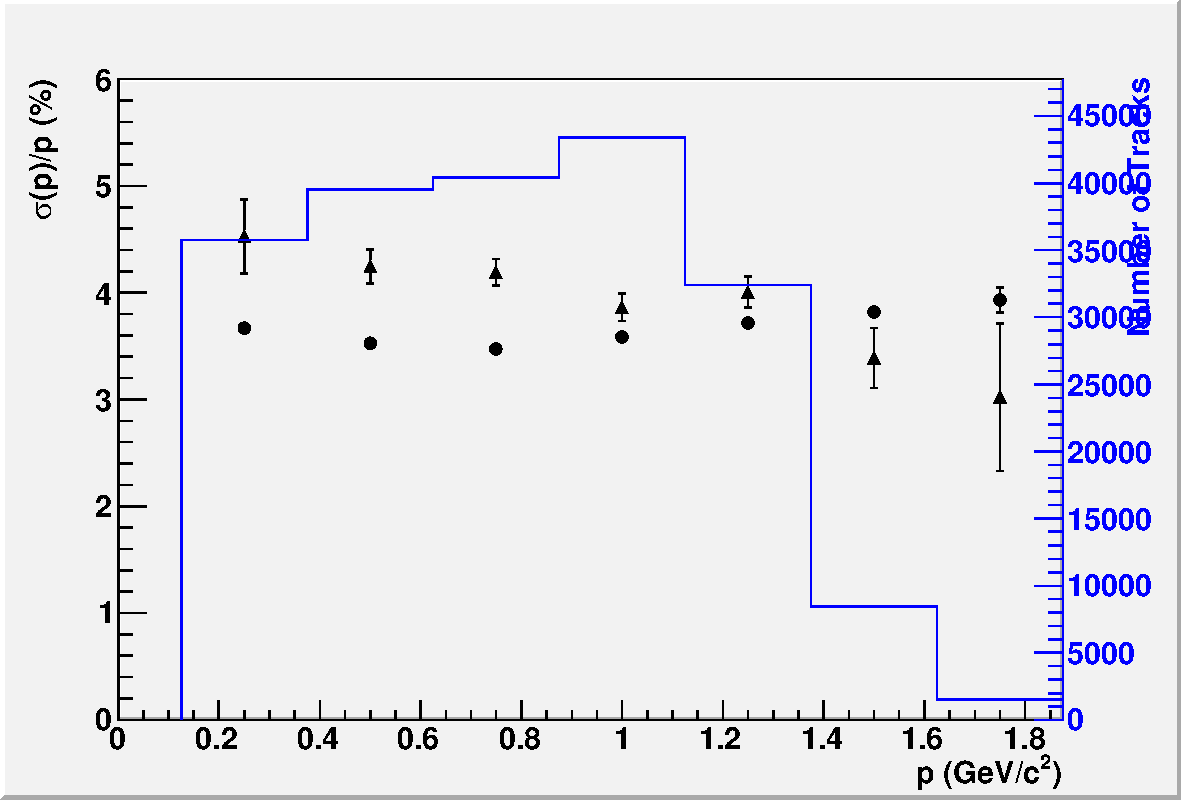
\includegraphics[scale=0.8]{performance/tracking_performance/momResvsMom.pdf}
\caption{  Fractional momentum resolution versus momentum. } 
\label{fig:trkmom}
\end{figure}


One quantity we use to determine track quality is the distance of closest approach (DOCA) 
to the beam axis.  We use this instead of the DOCA to the target beam spot since we are 
interested in long-lived decays and tracks from those will not point back to the target. 
We separate the distance into the bend plane (XOCA) and non-bend plane (YOCA) distances.  
Below, in Figure \ref{fig:doca}, is the resolution of these quantities as function of momentum.  
The resolution is, on average, about 100$\mu$m 300 $\mu$m) 
in the non-bend (bend) direction but increases significantly at low momentum.  The position 
resolution for tracks with one or more bad hits is somewhat worse, depending on which layer 
the bad hit is.  Tracks with bad hits in 
layers 1 or 2 are a major contribution to the tail of the vertex position distribution. 
    
For long lived A' decays, the position of the decay vertex is an important discriminating 
variable.  The dominant background to A' production is radiative events which originate 
in the target. Distinguishing A' decays from the background therefore depends on the vertex 
resolution and in particular on the tails of the vertex distribution. In order to study 
the tails, we use large samples of A' events decaying promptly overlaid on top of the 
simulated beam background events.
   
\begin{figure}
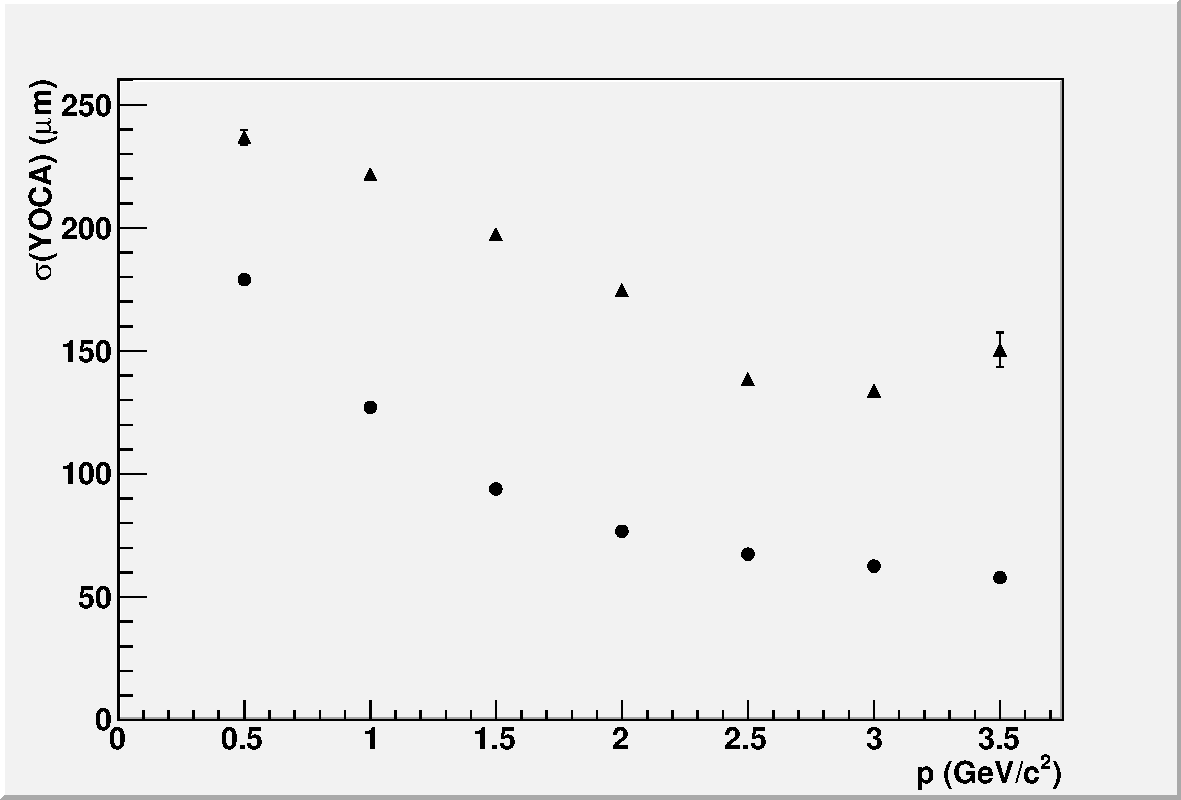
\includegraphics[scale=0.4]{performance/tracking_performance/yoca-MomResolution.pdf}
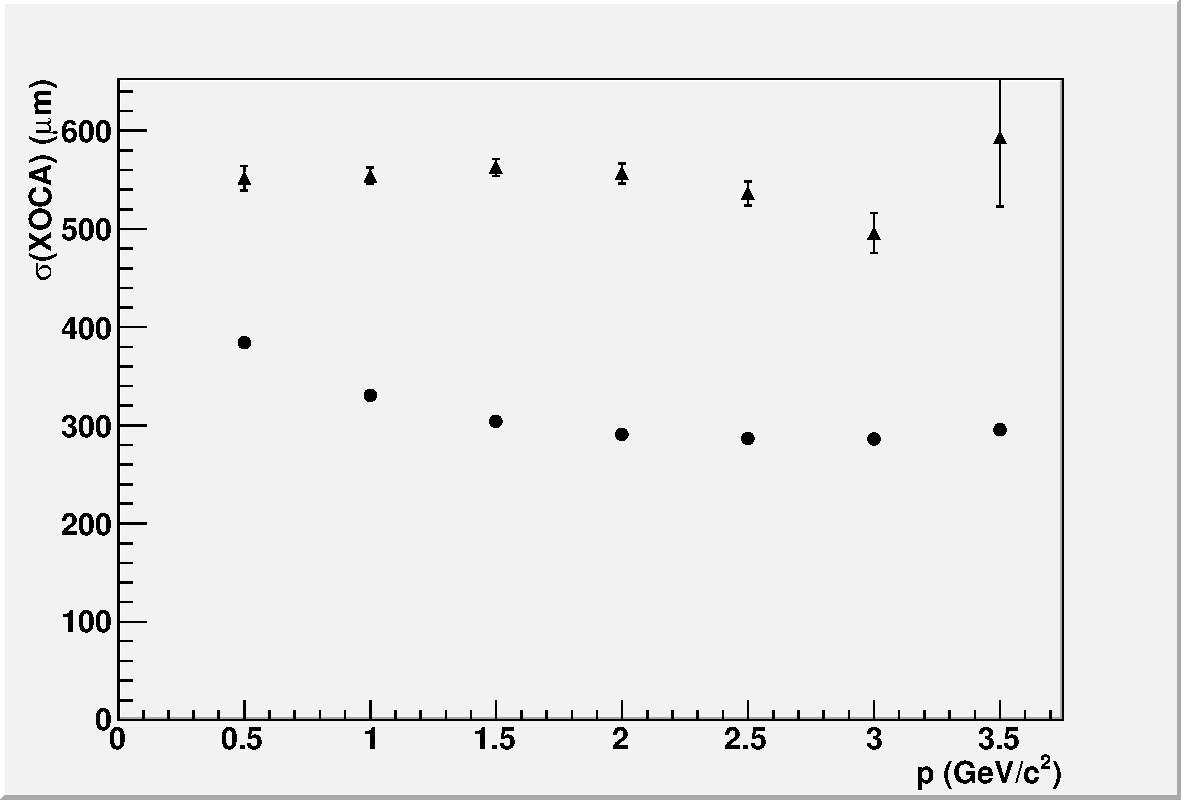
\includegraphics[scale=0.4]{performance/tracking_performance/xoca-MomResolution.pdf}
\caption{The resolution of the position of closest approach to the beam axis 
versus track momentum in the (left) non-bend direction and (right) bend direction.}
 \label{fig:doca}
\end{figure}

Each pair of oppositely charged tracks is fit to a common vertex using a Kalman filtering 
method first suggested by Billoir \cite{bf}, \cite{bq} and used in many experiments.  The method 
uses the measured helix parameters and their correlations to determine the most likely 
decay position of the A' and also returns fitted momenta for each particle.  We actually 
fit each pair twice with different hypotheses of their origin.  We constrain either 
the vertex to be consistent with an A':

\begin{itemize}
\item which originates in the 200$\mu$m $\times$ 40$\mu$m beamspot at the target, and moves off 
in the direction given by the measured A' momentum.  This fit will be used for the vertexing search.  
\item which originates and decays at the target within the 200$\mu$m $\times$ 40$\mu$m beamspot.  
This fit will be used for the bump-hunt only search.  
\end{itemize}

For each electron/positron pair reconstructed in the tracker, we compute the invariant mass based 
on the fitted momenta of the tracks.  The mass resolution depends on the invariant mass of the pair 
and is shown in Figure \ref{fig:massres}.  The closed circles  in Figure \ref{fig:massres} shows the improvement 
in the resolution for the second fit, where the decay is assumed to occur in the target.  

\begin{figure}
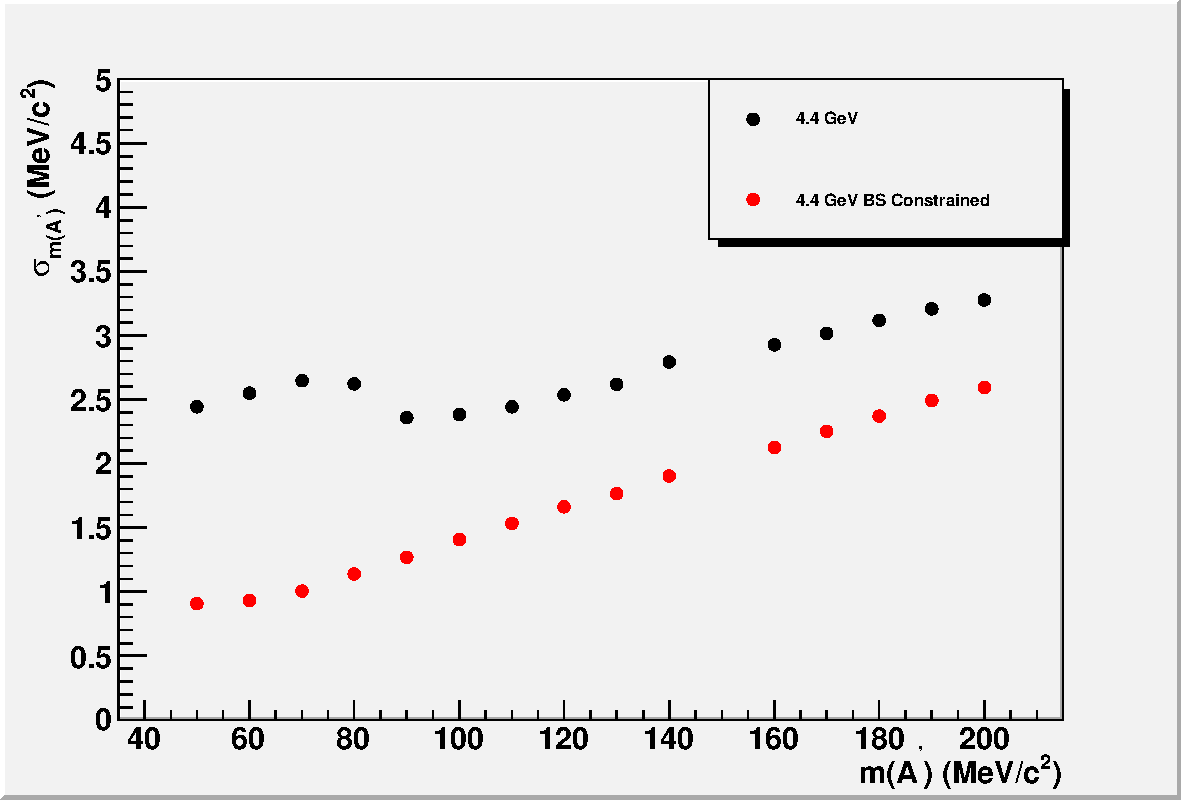
\includegraphics[scale=0.8]{performance/tracking_performance/massRes-4pt4.pdf}
\caption{The gaussian width of the mass distributions (MeV/c2) vs generated A' mass (MeV/c2). 
 The open circles are the resolutions when the decay is constrained to the target beamspot 
and the closed circles are without this constraint.    }
label{fig:massres}
\end{figure}



Even for prompt decays, the z vertex position (Vz) distribution of all reconstructed $e^+e^-$ pairs
  (solid black histogram, Figure \ref{fig:vtxResolutionRaw}) shows a long tail, still significant beyond 5cm.   
This tail is primarily comprised of events where one or both of the tracks use one or 
more bad hits.  Fortunately there are a number of quantities we can use to minimize the tails.  
Namely, for purposes of this proposal, we make the following cuts:

\begin{itemize}
\item The $\chi^2$  of each track is less than 20
\item The total momentum of the A' candidate is less than the beam energy
\item A very loose cut on the reconstructed vertex position $|V_x|<400\mu$m and $|V_y|<400\mu$m
\item The clusters in layer 1 of each track must be isolated from the next closest cluster by at least 500 $\mu$m 
\item A $\chi^2$ cut on the vertex fit of less than 5.
\end{itemize}

The vertex resolution depends on the invariant mass of the particles being vertexed. 
Lower masses have worse Gaussian resolutions as shown in Figure \ref{fig:vtxResolutionGauss}.  This is expected 
since the error on the opening angle ($\theta$), due to multiple scattering, scales like: 
 $\sigma (\theta )/\theta \sim (1/E)/(m/E) \sim 1/m$.
 
Figure \ref{fig:vtxResolutionRaw} shows the vertex resolution for samples of 80 MeV and 160 MeV A' events. 
The cuts above remove almost all of the tail past ~1.5cm (points with errors in Figure \ref{fig:vtxResolutionRaw}) 
while retaining ~50\% of the $e^+e^-$ pairs from the A' candidate. The events on the tail are 
enhanced with vertices where there are one or more bad hits on the track (represented by the 
blue histogram in Figure \ref{fig:vtxResolutionRaw}), although there is still a contribution from well-reconstructed 
tracks.  The rejection of tracks with bad hits depends strongly on the precision of the virtual A' 
trajectory, which in turn depends on the size of the beamspot. Having a beamspot significantly 
smaller than the intrinsic tracker resolution, 100$\mu$m in the non-bend and 300$\mu$m in 
the bend directions, is important.  

In practice, there is much more we can do to clean up the vertex and mass resolution both at 
the track level (e.g. remove hits that are clearly from scattered beam electrons) and at 
the vertex level.  These will be pursued in the near future.

\begin{figure}
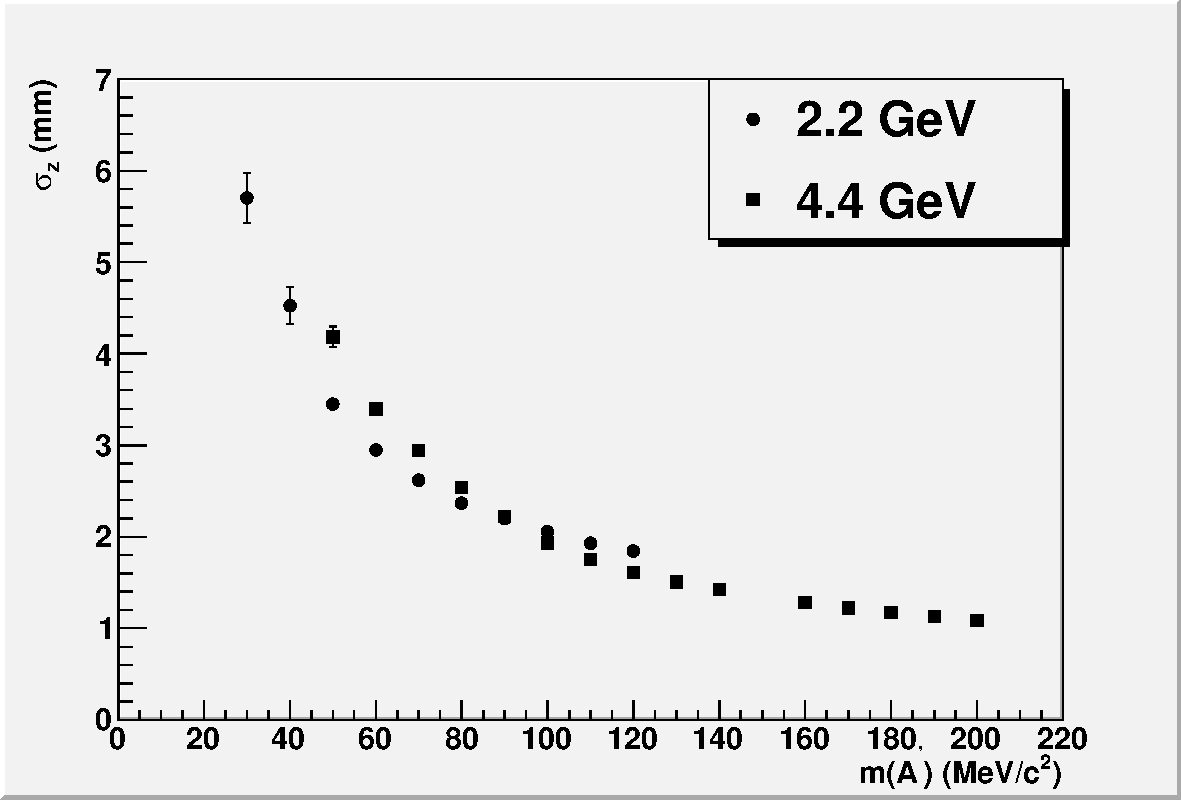
\includegraphics[scale=0.8]{performance/tracking_performance/vertexRes-4pt4-2pt2.pdf}
\caption{ The Gaussian resolution dependence versus $A^\prime$ mass for signal-only events.   }
\label{fig:vtxResolutionGauss}
\end{figure}
   

\begin{figure}
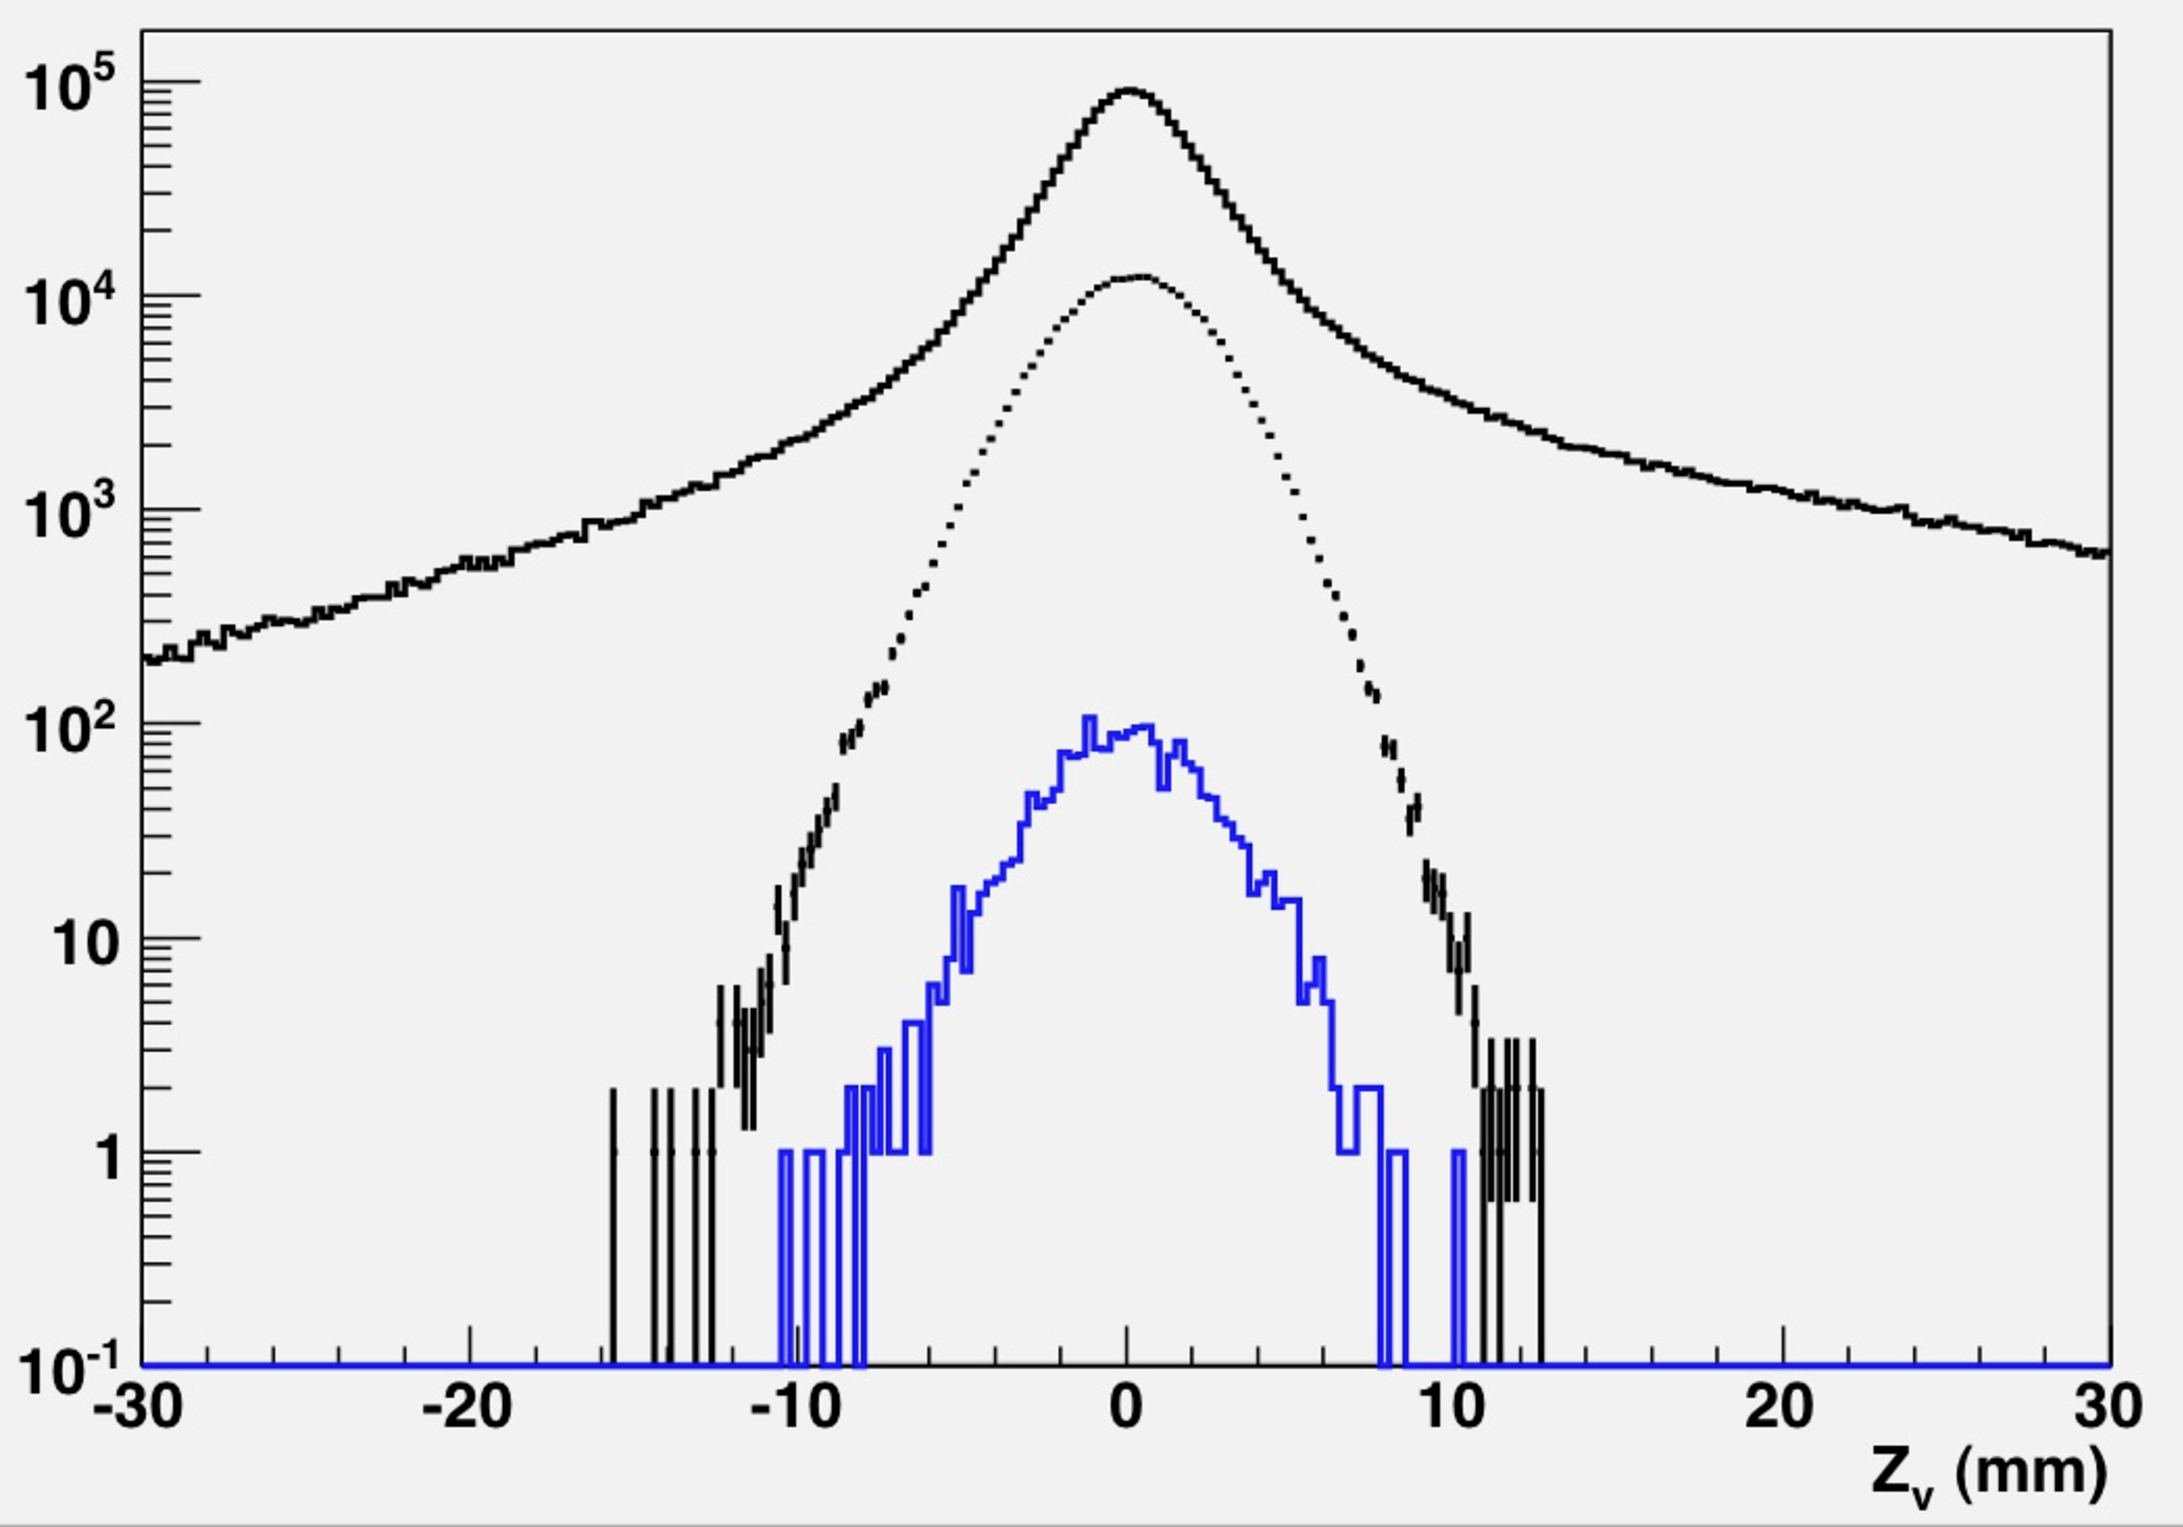
\includegraphics[width=0.8\textwidth]{performance/tracking_performance/v80.pdf}
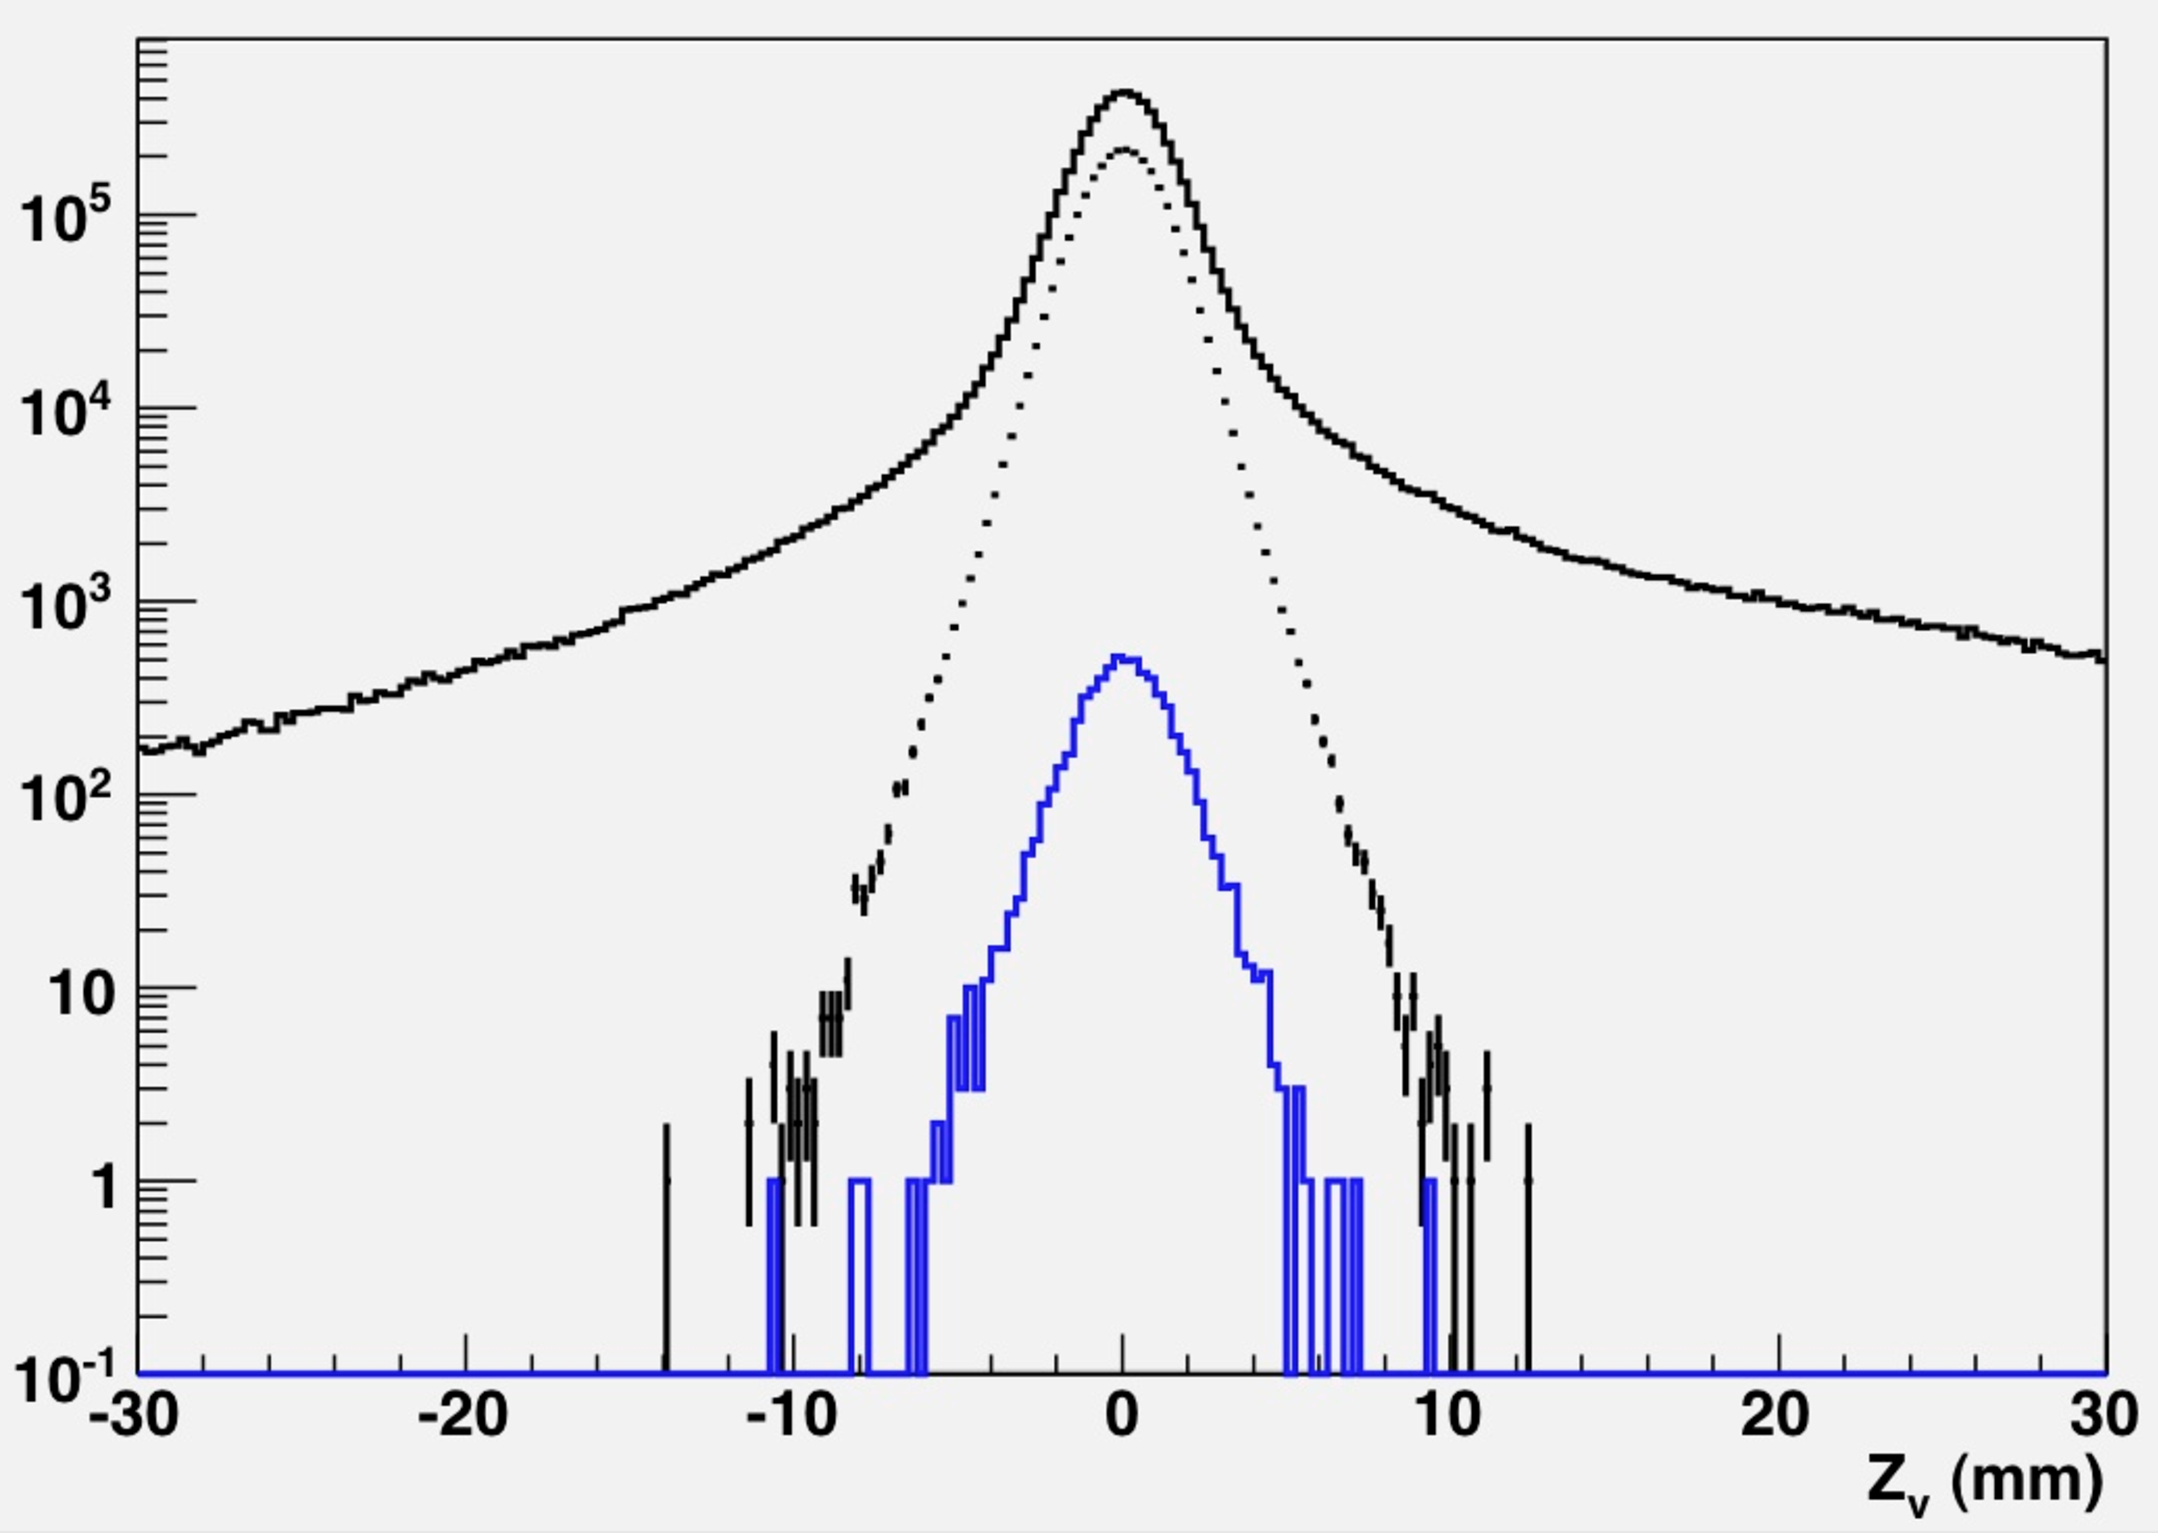
\includegraphics[width=0.8\textwidth]{performance/tracking_performance/v160.pdf}
\caption{Distribution of the reconstructed vertex position along the beam axis for 
4.4GeV 80MeV (top) and 160MeV (bottom) A' events before (solid black) and after (points 
with errors) selection.  The blue histogram shows the distribution for pairs that have 
at least one bad hit after selection.    }
\label{fig:vtxResolutionRaw}	
\end{figure}
  
\bibliographystyle{unsrt}
\begin{thebibliography}{99}
\bibitem{bf}
P. Billoir, R. Fruhwirth, and M. Regler, Nucl. Instr. And Meth. {\bf A241}, 115 (1985). 

\bibitem{bq}
P. Billoir and S. Qian, Nucl. Instr. And Meth. {\bf A311}, 139 (1991). 

\end{thebibliography}



%\subsection{Cluster reconstruction}

%\subsection{Muon identification}

